%% ****** Start of file aiptemplate.tex ****** %
%%
%%   This file is part of the files in the distribution of AIP substyles for REVTeX4.
%%   Version 4.1 of 9 October 2009.
%%
%
% This is a template for producing documents for use with 
% the REVTEX 4.1 document class and the AIP substyles.
% 
% Copy this file to another name and then work on that file.
% That way, you always have this original template file to use.

%\documentclass[aip,graphicx]{revtex4-1}
%\documentclass[aip,reprint]{revtex4-1}

%\usepackage{graphicx}

%\draft % marks overfull lines with a black rule on the right
%\documentclass[pre,aps,floatfix,authordate1-4,twocolumn]{revtex4-1}
%\documentclass[pre,aps,floatfix,authordate1-4]{revtex4-1}

\documentclass[aip,jcp,twocolumn]{revtex4}
%\documentclass[aip,jcp]{revtex4}
%\documentclass{article}



%\documentclass[aps,prl,preprint,groupedaddress]{revtex4}

\usepackage{rotating} 
\usepackage{times}
\usepackage{graphicx}
\usepackage{setspace}
\usepackage{amsmath}
\usepackage{epstopdf}
\usepackage[obeyFinal]{easy-todo}
\usepackage{csquotes}
\usepackage{mhchem}
\usepackage{chemfig}

%\usepackage{markdown} 

\begin{document}

% Use the \preprint command to place your local institutional report number 
% on the title page in preprint mode.
% Multiple \preprint commands are allowed.
%\preprint{}

\title{Accurate binding of sodium and calcium to phospholipid bilayers by effective inclusion of electronic polarization} %Title of paper

% repeat the \author .. \affiliation  etc. as needed
% \email, \thanks, \homepage, \altaffiliation all apply to the current author.
% Explanatory text should go in the []'s, 
% actual e-mail address or url should go in the {}'s for \email and \homepage.
% Please use the appropriate macro for the type of information

% \affiliation command applies to all authors since the last \affiliation command. 
% The \affiliation command should follow the other information.

\author{Josef Melcr}
\author{Hector Martinez-Seara Monne}
\affiliation{Institute of Organic Chemistry and Biochemistry,
Academy of Sciences of the Czech Republic, 
Prague 6, Czech Republic}
\author{Ji{\v r}{\' i} Kolafa}
\affiliation{Department of Physical Chemistry, Institute of Chemical Technology, Prague 6, Czech Republic}
\author{Pavel Jungwirth}
\affiliation{Institute of Organic Chemistry and Biochemistry,
Academy of Sciences of the Czech Republic, 
Prague 6, Czech Republic}
\affiliation{Department of Physics, Tampere University of Technology, P.O. Box 692, FI-33101
Tampere, Finland}

\author{O. H. Samuli Ollila}
\email[]{samuli.ollila@helsinki.fi}
%\homepage[]{Your web page}
\affiliation{Institute of Organic Chemistry and Biochemistry,
Academy of Sciences of the Czech Republic, 
Prague 6, Czech Republic}
\affiliation{Institute of Biotechnology, University of Helsinki}


% Collaboration name, if desired (requires use of superscriptaddress option in \documentclass). 
% \noaffiliation is required (may also be used with the \author command).
%\collaboration{}
%\noaffiliation

\date{\today}

\begin{abstract}
  % insert abstract here
Binding affinities and stoichiometries of Na$^+$ and Ca$^{2+}$ ions to phospholipid
bilayers are of paramount significance in the properties and functionality of cellular
membranes. For example, possible accumulation of ions at the membrane interface determines
the interaction affinity with charged species. Current estimates of binding affinities and
stoichiometries of cations are, however, controversial due to limitations in the available experimental and
theoretical methods. Experimentally one can assess these parameters by titrating
several membrane properties as a function of the ion concentration. However, the
interpretation of the experiments relies on theoretical models, which give
the best idealization of the ion binding as the direct experiments are not available. 
Classical molecular dynamics (MD) simulations provide details of the ion binding process with atomistic
resolution, therefore offering all the necessary information to interpret
experimental data without the need to resort to simplified models. However, the accuracy
of the available lipid models when interacting with ions is not sufficient for
such interpretation. In this work, we improve the binding details of Na$^+$ and Ca$^{2+}$ ions to the
1-Palmitoyl-2-oleoyl-phosphatidylcholine (POPC) bilayer by implicitly including electronic
polarization as a mean field correction, known as the electronic continuum correction (ECC).
This is applied to the partial charges of a selected state of the art POPC lipid model for MD simulations.
Our improved ECC-POPC model reproduces not only the
experimentally measured structural parameters for the ion-free membrane, but also the
response of lipid headgroup to a bound positive charge, and the binding affinities of 
Na$^+$ and Ca$^{2+}$ ions. With our new model we also observe negligible binding of Na$^+$ ions to POPC
bilayer and stronger interactions of Ca$^{2+}$ primarily with phosphate oxygens 
, which are in agreement with the previous interpretations of the experimental spectroscopic data.
On the other hand, the new model results in Ca$^{2+}$ ions forming complexes with one to three POPC molecules with almost
equal probabilities, suggesting more complex binding stoichiometry than simple models
previously used to interpret the NMR data.
The results of this work pave the way to quantitative MD simulations of complex
biochemical systems with realistic electrostatic interactions in the vicinity of cellular
membranes.
\end{abstract}

%\pacs{}% insert suggested PACS numbers in braces on next line

\maketitle %\maketitle must follow title, authors, abstract and \pacs

% Body of paper goes here. Use proper sectioning commands. 
% References should be done using the \cite, \ref, and \label commands


% Here I write pseudo-article statements that will make the main argument.
% Beautiful polished sentences will be formed only afte we agree on these basic things
\section{Introduction}
Ion interactions with cellular membranes play a key role in critical biological processes~\cite{seelig90,cevc90}. Ions, especially multivalent cations, modify general properties of the membrane which ultimately modulate their embedded transmembrane proteins~\cite{cevc90,tocanne90, pabst07}. Ions also have a more direct effect by modulating lipid--, protein--, and sugar--lipid interactions at the membrane surface. For example, Ca$^{2+}$  is crucial in neural signal propagation. It promotes membrane fusion by bridging lipids in the vesicles carrying neurotransmitters and the neuron synapsis membrane~\cite{REF}. Ca$^{2+}$ also participates in the T-cell receptor activation. It induces the detachment of the positively charged cytosolic tails of the CD3 protein complex from the negatively charged intracellular membrane making it accessible for Lck protein~\cite{Shi2013}. A final example involving sugar-lipid interactions mediated by ions is that Ca$^{2+}$ can modulate the presentation of the sugars found in the PI(4,5)P$_2$ lipid which ultimately modulates phospholipase C delta 1 pleckstrin homology domain (PLC $\delta$1-H)~\cite{Bilkova2017Calcium}. Interestingly, this modulation is lost when using Mg$^{2+}$ instead of Ca$^{2+}$ illustrating the selectivity of these processes towards particular ions. Despite our increasing understanding of the role of ions in cell membrane-related processes the exact molecular details of the mechanisms behind such processes remain elusive.

Direct measurements of ion-membrane interactions in real biological systems are difficult. Simplified lipid bilayers are often used instead as entry-level models to shed light on the role of ions in complex biological membranes~\cite{scherer87,seelig90,cevc90}. For this reason, interactions of biologically relevant cations, especially Na$^+$ and Ca$^{2+}$, with zwitterionic phosphocholine (PC) bilayers have been widely studied in experiments~\cite{akutsu81, altenbach84, seelig90, cevc90, tocanne90, binder02, pabst07, uhrikova08} and classical MD simulations~\cite{bockmann03, bockmann04, Berkowitz12, melcrova16, javanainen17}. The details of ion binding are, however, not fully consistent in the literature. Non-invasive spectroscopic methods, like nuclear magnetic resonance (NMR), scattering, and infrared spectroscopies mainly suggest that Na$^+$ ions exhibit negligible binding to PC lipid bilayers. On the contrary, Ca$^{2+}$ is observed to specifically bind to a couple of PC molecules using their phosphate groups~\cite{hauser76, hauser78, herbette84, akutsu81, altenbach84, binder02, pabst07, uhrikova08}. On the other hand, in general atomistic resolution molecular dynamics (MD) simulation models predict a stronger binding for the cations~\cite{catte16}. For example, simulations report Na$^+$ accumulating in the lipid interface~\cite{bockmann03} or Ca$^{2+}$ binding up to 4 PC lipids simultaneously, including not only interactions with phosphates but also with carbonyl oxygens~\cite{bockmann04, melcrova16, javanainen17}.
%{\color{red} Also, several experiments have also been interpreted to support the predictions from earlier MD simulations~\cite{bockmann03, vacha09a}. \todo{remove? Why we need this?}}

Recent studies within the NMRlipids project (\url{nmrlipids.blogspot.fi})~\cite{catte16} made an attempt to resolve these apparent controversies. A direct comparison of ion binding affinities to PC bilayers between simulations and experiments was performed using the electrometer concept~\cite{seelig87}. Namely, the changes in NMR order parameters of the headgroup upon addition of ions is directly compared to the MD simulations results. Analyzing massive amounts of data collected by the Open Collaboration method, it was concluded that the accuracy of the current state of the art lipid models for MD simulations is not sufficient for a detailed interpretation of the interactions of cations with PC lipid bilayers~\cite{catte16}.



%\todo{PAVEL: introduce previous theoretical work that discusses cation binding to POPC w.r.t. its specific moiteties, e.g. Lukas' paper}.

%While relative binding affinity of different ions in PC lipids is agreed to follow Hoffmeister
%series, the molecular details of binding and binding energetics are

%The binding details, like binding sites and stoichiometry are not yet fully
%resolved but interpretation of NMR and scattering experiments suggest that one
%Ca2+ interacts mainly with the choline groups \cite{hauser76,hauser78,herbette84} of two
%phospholipid molecules \cite{altenbach84}.

In this work, we improve the cation binding of a POPC bilayer in MD simulations via the implicit inclusion of the electronic polarizability in the polar region of phospholipids. For this, we apply a simple mean-field electronic continuum correction (ECC)~\cite{leontyev11} which implies scaling the partial charges of the atoms to account for the missing electronic polarizability in MD simulations~\cite{leontyev11}. Such an approach has been previously shown to improve the behavior of ions in bulk water simulations ~\cite{jungwirth17-new-paper-to-be-published, Pluharova2014, kohagen14, kohagen16}. As a starting template for our POPC model, we will use the Lipid14~\cite{dickson14}. This force field provides one of the best available descriptions of cation binding \cite{catte16}. The newly developed ECC-lipids model reproduces the experimentally
measurable structural parameters of an ion-free POPC lipid bilayer with the accuracy comparable to the best state of the art lipid models, while improving the membrane binding affinities significantly to sodium and calcium cations.

%Since the cation binding affinity and the headgroup 
%order parameter changes are in good agreement with experiments
%in the proposed ECC-lipids, it can be used to interpret the
%related structural changes and ion binding stoichiometry.
%New lipid models with correct ion binding affinity in lipid
%bilayers are necessary in applications of 
%MD simulations with physiological salt conditions. 
%The overestimated cation binding in the current lipid models \cite{catte16}
%may lead to significant artefacts in MD simulations. For example,
%articifially positively charged membranes overestimate interactions
%with biomolecules having opposite sign.


\section{Methods}

\subsection{Electronic continuum correction for lipid bilayers}\label{section:ecc}
The lack of electronic polarizability in standard MD simulation force fields has been considered a serious issue since the early days of lipid bilayer simulations. In this work, we circumvent the demanding explicit inclusion of electronic polarization effects~\cite{lucas12, chowdhary13} by including the electronic part of polarizability in lipid bilayer simulations implicitly via the electronic continuum correction (ECC)~\cite{leontyev11}. Technically, this is similar to the phenomenological charge-scaling applied in earlier studies of surfactants, lipids or ionic liquids \cite{jonsson86, egberts94, beichel14}. However, the present concept of ECC is physically well justified and rigorously derived~\cite{leontyev09, leontyev10, leontyev11, leontyev14}.

According to ECC, the electronic polarizability can be modeled in non-polarizable MD by effectively embedding the ions in a homogeneous dielectric continuum with a dielectric constant $\epsilon_{el}$, which is the electronic part of the dielectric constant of the medium~\cite{leontyev11}. Following Coulomb's law,  ECC can be directly incorporated by scaling the charges with a constant scaling factor of $f_q = \epsilon _{el} ^{-1/2}$, giving
\begin{equation}
Q^{ECC} = f_q \cdot Q
\end{equation}
for the ECC corrected charges in simulation. 
Given that the  high frequency dielectric constant of water is $\epsilon _{el} = 1.78$ (\textit{i.e.,} the square of the refraction index), the scaling factor for ions in water is roughly $f_q \approx 0.75$. This scaling factor successfully improves the accuracy of simulations of solvated ions \cite{kohagen14, kohagen16, REF}, when quantitatively compared with neutron scattering data \cite{kohagen14,kohagen16, Pluharova2014}.
It is important to note that the 
high frequency dielectric constant 
is around 2 for almost any biologically relevant environment \cite{some_original_work, leontyev11}.
The dielectric discontinuity in a lipid bilayer arises
from the orientational polarization of the molecules. 
Thus, the same correction for the electronic polarizability can be 
applied throughout the lipid bilayer interface.



While using a scaling factor of $f_q = 0.75$ for ions in water is well justified in the ECC theory \cite{Leontyev2011}, it is not clear whether the same factor should be applied to partial charges used to describe molecules in MD models, e.g., lipids in our case. Unlike the total charge of an ion, atomic partial charges within molecules are not physical observables. Several schemes exist for the assignment of partial charges for biomolecules~\cite{Hu2007}, where the restrained electrostatic potential method (RESP) is the most commonly used~\cite{RESP_paper, Singh1984}. Considering that water molecules are often included in RESP calculations or charges are refined to improve certain experimental observables, the electronic polarizability effect of the solvent is included in modern force fields to some extent~\cite{RESP_paper, Singh1984, jorgensen96, ipolq2013, benavides17}. Thus, the application of the ECC scaling factor, $f_q$, to the existing partial charges in molecules does not universally follow $f_q = \epsilon _{el} ^{-1/2}$. Instead, a consistent scaling factor would lie between the value of 0.75  (\textit{i.e.,} no electronic polarizability included in the original partial charges) and 1 (\textit{i.e.,} electronic polarizability fully included in the original partial charges). 

Here we develop ECC-POPC lipid model that accurately describes the binding 
of sodium and calcium ions to the lipid bilayer. 
The Lipid14~\cite{dickson14} force field parameters 
(available in a Gromacs format from Ref. \citenum{lipid14files}) were used as a starting 
point. 
This model provides the best response of the head group to ions among the available 
lipid models (see Figs.~2~and~5 in Ref.~\citenum{catte16}). Additionally, the Lipid14 model 
has a relatively realistic head group, glycerol backbone, and acyl chain structure~\cite{dickson14,botan15}.
We applied the ECC correction 
to the Lipid14 model of POPC by scaling of 
partial charges of the head group, glycerol 
backbone, and carbonyl regions. 
These are the polar parts of phospholipids which can 
contribute to the cation binding. 

To reproduce the experimental ion binding affinities,
we scanned the optimal interval for the scaling factor, $f_q~\in~(0.75, 1.0)$.
In general, scaling down the partial charges reduces the ion binding affinity 
and the experimentally measurable head group order parameter response to the bound charge~\cite{akutsu81, altenbach84, scherer89}. We found an optimal value $f_q = 0.8$, which is only slightly higher than the theoretical one ($f_q=0.75$). Directly applying the 0.8 scaling to the partial charges of the head group, the glycerol backbone, and the carbonyls reduces the area per lipid to 60~\AA$^2$. This area is smaller than the original in Lipid14 model ($65.6 \pm 0.5$~\AA$^2$)~\cite{dickson14} and the experimental value (64.3~\AA$^2$) \cite{kucerka11}. The decrease of the area per lipid arises from a reduced hydration of the lipid head group region after scaling charges which effectively reduces head group polarity. 
We solve this difficulty by reducing the effective radii of the modified atoms by lowering the $\sigma$ parameters in the Lennard-Jones potential by a factor of $f_\sigma = 0.89$. The same solution was taken for the ECC-ions in aqueous solvent \cite{kohagen14, kohagen16, Pluharova2014}. After reducing the $\sigma$ parameters, the area per molecule is restored to the experimental value (Table~\ref{tab:apls}). 




\subsection{Electrometer concept} \label{section:electrometer}
Comparing MD simulation to NMR experiments, we can validate the simulation ion binding affinity to lipid bilayers using the ''electrometer concept''~ \cite{seelig87, catte16}. This method relies on the experimental observation that the C-H bond order parameters of $\alpha$ and $\beta$ carbons in a PC lipid head group (Fig.~\ref{simVSexpNOions}) are proportional to the amount of charge bound per lipid~\cite{seelig87}. Comparing this response is an excellent way to validate force fields as both NMR and MD can accurately determine order parameters ~\cite{catte16, ollila16}. The order parameters for all C-H bonds in lipid molecules can be accurately measured using $^2$H NMR or $^{13}$C NMR techniques \cite{ollila16}. From MD simulations the order parameters can be calculated using the definition
\begin{equation}\label{OP}
S_{\rm CH}=\frac{3}{2}\langle \cos^2\theta -1 \rangle,
\end{equation}
where $\theta$ is the angle between the C-H bond and membrane normal. Angular brackets point to the average over all sampled configurations.

The relation between the amount of the bound charge per lipid, $X^\pm$, and the head group order parameter change, $\Delta S_{\rm{CH}}^{i}$, is empirically quantified as~\cite{seelig87,ferreira16}
\begin{equation}\label{OPchangeEQ}
\Delta S_{\rm{CH}}^{i}= S_{\rm{CH}}^{i}(X^\pm)-S_{\rm{CH}}^{i}(0) \approx m_i \frac{4 }{3\chi}X^\pm,
\end{equation}
where $i$ refers to either $\alpha$ or $\beta$ carbon, $S_{\rm{CH}}^{i}(0)$ denote the order parameter in the absence of bound charge, $\chi$ is the quadrupole coupling constant ($\chi \approx$\,167\,kHz), and $m_i$ empirical experimental constant depending on the valency and position of the bound charge.


The measured change of the order parameter depends both on the head group response to the bound charge and on the amount of the bound charge (\textit{i.e.,} $m_i$ and $X^\pm$ in Eq.~\ref{OPchangeEQ}, respectively).  The empirical factor $m_i$ has to be adequately quantified before the electrometer concept can be used to analyze the binding affinities. This calibration has been done experimentally for a wide range of systems~\cite{seelig87, beschiasvili91}. To calibrate the response of the head group order parameter to the bound charge in simulations, we use experimental data for a strong cationic surfactant dihexadecyldimethylammoniumbromide  (DHAB) bilayer~\cite{scherer89}. DHAB\\[0.5cm]
%\vspace{0.5cm}
\chemfig{
  -[:0,3.5,,,draw=none]\chemabove{N}{\scriptstyle\oplus} (-[:150]H_3C)(-[:210]H_3C)(-[:330]{(}CH_2{)}_{15}-CH_3)(-[:30]{(}CH_2{)}_{15}-CH_3)
}  
\vspace{0.5cm} \\
is a cationic surfactant having two acyl chains and bearing a unit charge in the hydrophilic end. Thus, it is expected to locate in the bilayer similarly to the phospholipids, and its molar ratio then gives directly the amount of bound unit charge per lipid $X^\pm$ in these systems~\cite{scherer89}.

\subsection{Salt concentrations and binding affinity}
NMR experiments report the used salt concentrations in two different ways when measuring head group order parameters. Some use the salt concentrations in water before solvating the lipids~\cite{akutsu81} while others use atomic absorption spectroscopy and report the salt concentration in the supernatant after the solvation of lipids~\cite{altenbach84}. In this work, we use the latter definition. In particular, we measure the salt concentration in the aqueous bulk region as that at the farthest point from the lipid bilayer in the aqueous phase. Notice that this definition differs from the one used by Catte et al.~\cite{catte16} where the former definition is used. Although these two definitions vary when applied to Ca$^{2+}$, they do not affect significantly the conclusions of this work.

To quantify the ion binding affinities to a lipid bilayer, we calculate the relative surface excess of ions with respect to water, $\Gamma_{ion}^{water}$~\cite{chattorajBOOK}. Such a quantity compares the adsorption of ions to the adsorption of water molecules at the interface without the necessity of defining a Gibbs dividing plane between the membrane interior and the water bulk region. In our simulations, we only assume that the interface is located between the ion-free hydrophobic interior of the lipid bilayer and the aqueous region far from the membrane.  Such a setup and the above definition of bulk ion concentration provide a simple relation for the relative surface excess $\Gamma_{ion}^{water}$ for simulations of lipid bilayers,
 
\begin{equation}\label{surfexcess}
  \Gamma_{ion}^{water}=\frac{1}{2A_b} \left ( n_{ion} - n_{water} \frac{C_{ion}}{C_{water}} \right ).
\end{equation}
Here, $n_{water}$ and $n_{ion}$ are the total numbers of water molecules and ions in the system,
$C_{water}$ and $C_{ion}$ are their respective bulk concentrations in the aqueous phase,
and $A_b$ is the area of the unit cell in the membrane plane.
The total area of the interface is then twice the area of the membrane, i.e., $2A_b$,
because the bilayer has an interface at each of the two leaflets.



\subsection{Validation of lipid bilayer structure against NMR and scattering experiments}
The structures of lipid bilayers in simulations without ions were validated against NMR by calculating the order parameters for the C-H bonds and \mbox{x-ray} scattering experiments by the scattering form factors. NMR order parameters validate the structures sampled by the individual lipid molecules with atomic resolution. The simulated order parameters were calculated for all C-H bonds in lipid molecules from Eq. \ref{OP}. Scattering form factors validate the dimensions of the lipid bilayer (e.g., thickness and area per molecule). Form factors were calculated using

\begin{equation}
  F(q) = \int _{-D/2} ^{D/2} \left ( \rho_{el}(z) - \rho_{el}^s \right ) \cos (zq_z) \mathrm{d}z,
  %F(q) = \int _{-D/2} ^{D/2} \left ( \sum _\alpha f_\alpha (q_z) n_\alpha (z) - \rho _s \right ) \exp (izq_z) \mathrm{d}z,
\end{equation}

\noindent where $\rho_{el} (z)$ is the total electron density, $\rho_{el}^s$ is the electron density of the solvent far in the aqueous bulk, and $z$ is the distance from the membrane center along its normal with $D/2$ being half of the unit cell size.  




\subsection{Simulation details}

\subsubsection{Simulations of POPC bilayers with aqueous ions}
Simulations of a POPC bilayer in pure water or at varying salt concentrations consisted of 128 POPC molecules and approximately 50~SPC/E~water~\cite{Berendsen1987} molecules per lipid in an orthorhombic simulation box with periodic boundary conditions.  The chosen SPC/E water model, also used in the previous parametrization of ECC-ions \cite{jungwirth17-new-paper-to-be-published, kohagen16, Pluharova2014}, has a lowered dielectric constant, consistent with the ECC concept~\cite{leontyev11, leontyev14}.  We checked other water models (OPC \cite{Izadi14}, OPC3~\cite{Izadi16}, TIP3P~\cite{jorgensen83}, TIP3p-FB and TIP4p-FB~\cite{Wang2014}, and TIP4p/2005 \cite{Abascal2005}) to confirm the robustness of our approach (See SI). Sodium, calcium, and chloride ions were modeled as ECC-ions with parameters from Ref. \citenum{jungwirth17-new-paper-to-be-published, Pluharova2014}.  
% cite order: [Ca_2s, Na_s, Cl_2s] 
Scaled charges and van der Waals radii for atoms forming the POPC lipid are derived in this work starting from the Lipid14 force field~\cite{REF}. For comparison, simulations with unscaled charges were performed using the Lipid14 model~\cite{REF}, the TIP3p model for water \cite{jorgensen83}\todo{HECTOR: Do we compare this against scaled with SPC or TIP3P?}, and ion models by Dang and coworkers~\cite{smith94,chang1999,dang2006}. Simulation data for the Lipid14 model with \AA{}qvist ions~\cite{aqvist90} and TIP3P~\cite{jorgensen83} water models were taken directly from Ref.~\citenum{catte16}.  

MD simulations were performed using the GROMACS \cite{Abraham15} simulation package (version 5.1.4). The simulation settings employed in this work are summarized in Table \ref{tbl:mdpar}\todo{HECTOR: Is this the SI? If so we have to indicate it. Now reference is weird.}. The simulated trajectories and parameters files are available at \cite{??} \todo{To be uploaded to Zenodo}.



\subsubsection{Simulations of POPC bilayers with cationic surfactants}
The topology of dihexadecyldimethylammonium was created with the automated topology builder \cite{malde11}. The AmberTools program~\cite{amber} was then used to generate the Amber-type force field parameters. These parameters were then converted to the Gromacs format with the acpype tool \cite{acpype}. The partial charges were then manually modified in the non-scaled version~\cite{catte16} to approximately match similar segments in Lipid14 \cite{dickson14}. For simulation with ECC-POPC, the partial charges of the headgroup were scaled, i.e., $f_q=0.8$, and the $\sigma$ of the scale atoms reduced as in POPC-ECC.

The cationic surfactants were randomly mixed among the phospholipids to form bilayer structures with mole fractions of 10\%, 20\%, 30\%, 42\%, or 50\% of surfactant in the POPC bilayer. All these systems contained 50 POPC molecules per leaflet, 6340 TIP3P~\cite{jorgensen83} water molecules, and 6, 14, 21, 35, or 50 surfactants per leaflet.  Chloride counter ions were used in simulations, while bromide was the counter ion in the experiment \cite{scherer89}. For POPC either the Lipid14 or ECC-POPC model was used. The first 20~ns of the total simulation time of 200~ns was considered as an equilibration time and was omitted from the analysis. Sufficient lipid neighbor exchange occurred during the simulations. Further details for the unscaled simulations and the trajectories are in Ref.~\citenum{catte16}.

\todo{Provide the parameteres for ECC-surfactant somewere.}

\section{Results and Discussion}

\subsection{POPC membrane structure and dynamics}

\begin{figure}[tb!]
  \centering
  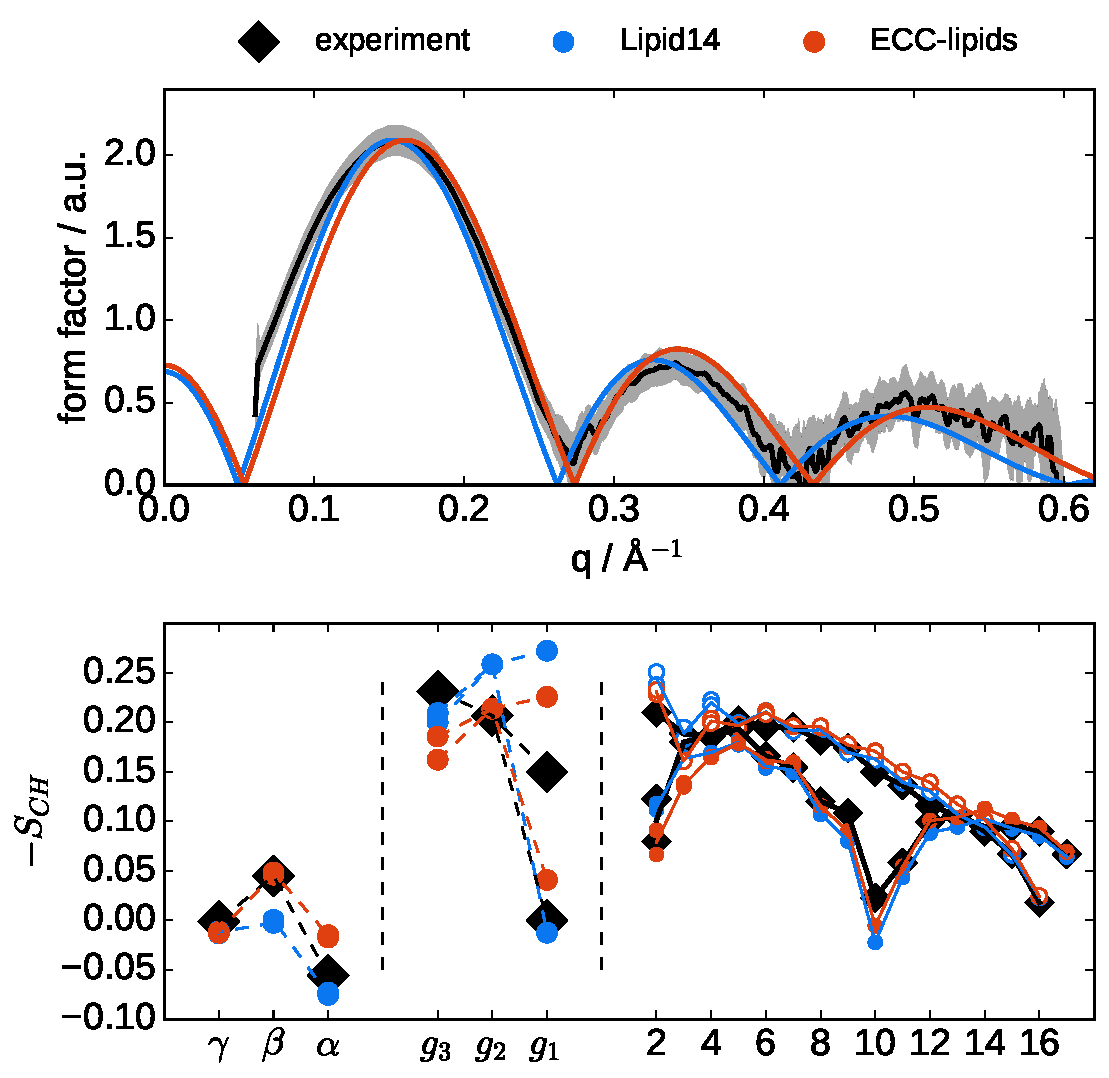
\includegraphics[width=8.2cm]{../Fig/ipython_nb/Order-parameters_form-factors_exp-L14-ECCL17_q80_sig89.pdf}
  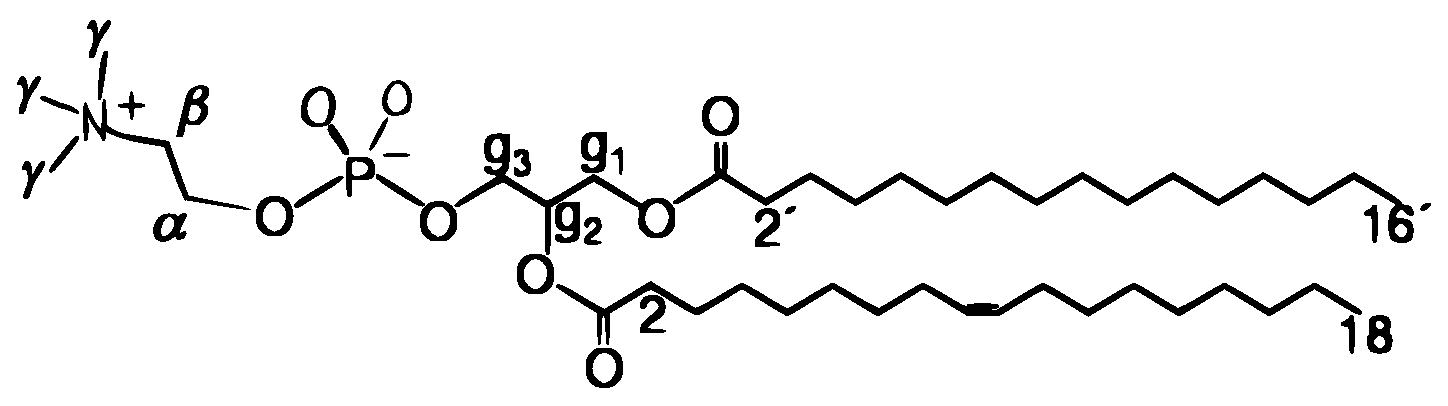
\includegraphics[width=7.4cm]{../Fig/POPCstructure.eps}
  %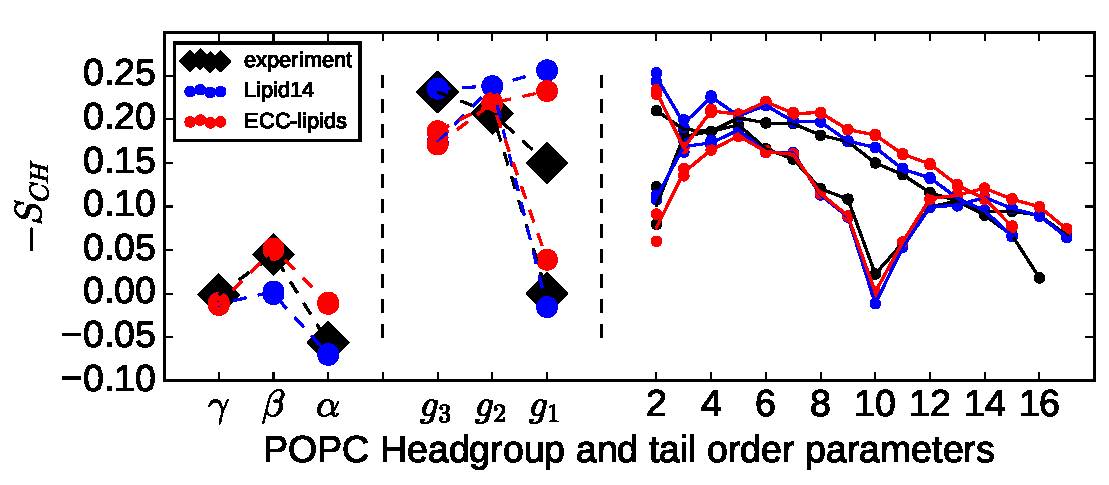
\includegraphics[width=8.0cm]{../Fig/ipython_nb/Order-parameters_exp-L14-ECCL17_q80_sig89.pdf}
  %\includegraphics[height=8.4cm,angle=-90]{../Fig/form-f_exp-l14-eccl17.eps}
  \caption{\label{simVSexpNOions}
    Top: X-ray scattering form factors from simulations with the Lipid14 \cite{dickson14} and
    the ECC-lipids models compared with experiments~\cite{Kucerka2011}.
    Middle: Order parameters of POPC head group, glycerol backbone and acyl chains 
    from simulations with the Lipid14 \cite{dickson14} and the ECC-lipids models
    compared with the experimental values from \cite{ferreira13}.
    The size of the markers for the head group order parameters correspond to
    the error estimate $\pm 0.02$ for experiments \cite{botan15,ollila16},
    while the error estimate for simulations is $\pm 0.005$.
    The size of the points for acyl chains are decreased by a factor of 3 to improve the clarity of the plot.
    Bottom: The chemical structure of POPC and the labeling of the carbon segments.
  } 
\end{figure}

\begin{table}[tb!]
  \caption{Values of the area per lipid (APL) of POPC bilayers without ions from the Lipid14 simulation
    ran in this work and from the literature \cite{dickson14}, from the ECC-lipids model, and from experiments.{ \color{red} HECTOR:Are we using here the same water model? If not is it fair the comparison considering the large changes observed in the SI table?}\label{tab:apls} }
  \begin{tabular}{l|c c}
    model          & APL (\AA$^2$)   & Temperature [K] \\
    \hline
    Lipid14                   & 65.1$\pm$ 0.6  &  300 \\
    Lipid14 \cite{dickson14}  & 65.6$\pm$ 0.5  &  303 \\
    \hline
    ECC-lipids                & {\color{red}63.2}$\pm$ 0.6  &  300       \\
    \hline
    experiment \cite{kucerka11} & 64.3  &  303    \\
    \hline
  \end{tabular}
\end{table}


First, we present results for bilayers in pure water.
The ECC-lipids and Lipid14 models both reproduce the experimental x-ray scattering form factors
of a POPC bilayer with a comparable accuracy in Fig.~\ref{simVSexpNOions}.
The area per lipid from the Lipid14 model is $\approx$1\AA{} larger than the
experimental value in Table~\ref{tab:apls}, while the value from the ECC-lipids model
is $\approx$1\AA{} smaller\todo{The 63.2 value does not appear in the SI table. There it is 62.2 but I'm not sure corresponds to the same system}. The values of the area per lipid of the ECC-lipids model show larger variations
when simulated with different water models (i.e., 62.2--66.8 \AA{}, see Table~\ref{tab:apls_si} in SI\todo{HECTOR: change to real reference in SI}),
while still being close to the experimentally reported values.
We can thus conclude that the ECC-lipids model reproduces the experimental dimensions of the POPC
lipid bilayer with accuracy comparable to that for another state of the art lipid models \cite{ollila16}.
%The optimal value for $f_\sigma$ was found by representing the overall membrane structure well
%by matching scattering form factors to experimental data~\cite{Petrache06, Kucerka08, Pabst10}.

Similarly, the acyl chain order parameters of the ECC-lipids model, as well as the Lipid14 model~\cite{dickson14}, agree with the experimental values within the error bars, as presented in Fig.~\ref{simVSexpNOions}. Notably, the experimentally measured forking and small order parameter values of $C_2$ segment in {\it sn}-2 chain are well reproduced by both models. This feature has been suggested to indicate that the carbonyl of {\it sn}-2 chain is directed towards the water phase, in contrast to the carbonyl in {\it sn}-1 chain, which would orient more along the bilayer plane~\cite{seelig75,schindler75,gawrisch92}. This arrangement may be a relevant feature for the ion binding details, which it is not fully reproduced by other available lipid models~\cite{ollila16}.
%This is expected as the ECC model does not modify the already highly optimized parameters of this region in Lipid14

The order parameters of the $\alpha$ and $\beta$ carbons in the headgroup are slightly larger in the ECC-lipids model than in the Lipid14 model, which is apparently related to the P-N vector orienting by about 7$^{\circ}$ more toward the water phase in the ECC-lipids model, see Fig.~\ref{OrderParameterCHANGESsurf}. Considering the available experimental evidence, it is not possible to suggest which of the two models provides more realistic headgroup orientation. The ECC-lipids model gives the $\beta$ carbon order parameter value closer to experiments than the Lipid14 model, while the opposite is true for the $\alpha$ carbon. The accuracy of both models in the glycerol backbone region is equally footed with any other state of art lipid model available in literature \cite{botan15}, see Fig.~\ref{simVSexpNOions}.


\todo{Dynamics check is missing: MSD (Hector/Joe)}

\subsection{Calibration of lipid electrometer:
            Response of POPC head groups to bound charge}\label{section:boundCHARGE}

\begin{figure}[tb!]
  \centering
  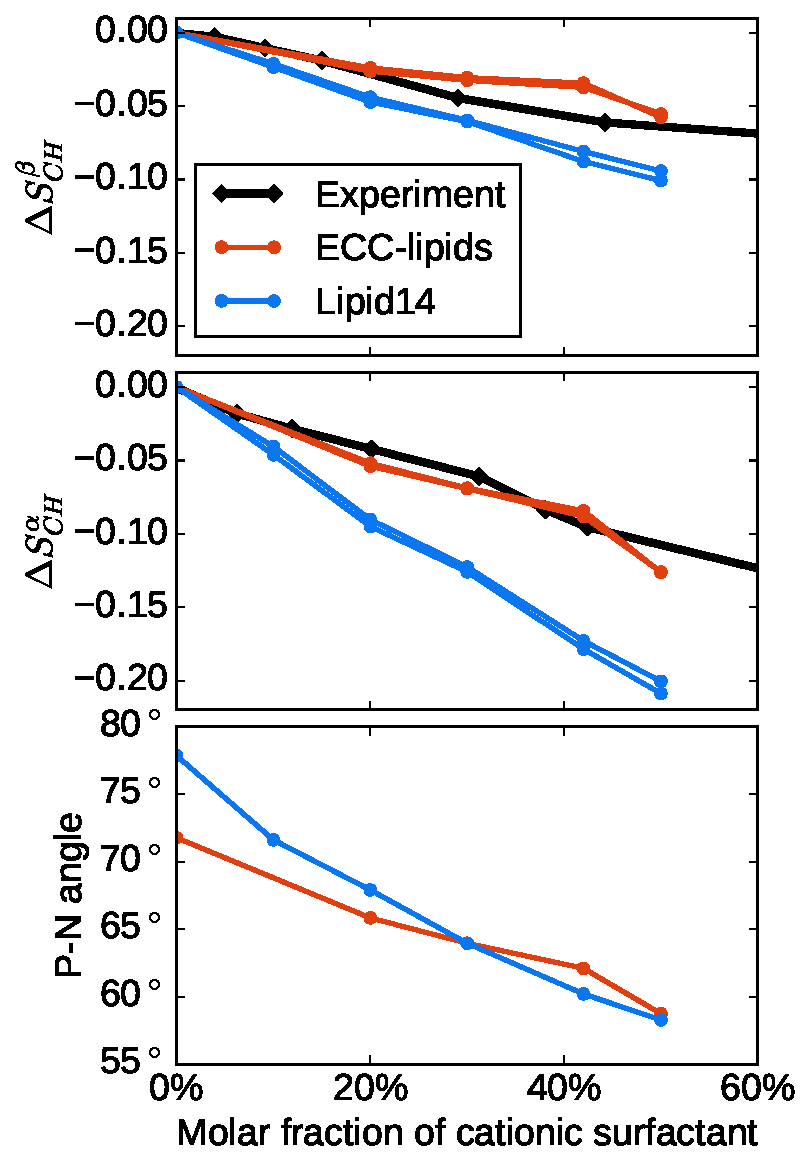
\includegraphics[width=8.0cm]{../Fig/ipython_nb/PN_angle_OrdPars-A-B_L14-ECCL17_q80_sig89_surf.pdf}
  \caption{\label{OrderParameterCHANGESsurf}
    The changes of headgroup order parameters and P-N vector orientation as a function of
    a molar fraction of the cationic surfactant dihexadecyldimethylammonium in a POPC bilayer
    from simulations and experiments \cite{scherer89}.
  }
\end{figure}

Before studying the sodium and calcium ion binding affinities, we have to quantify as reference the response of the headgroup order parameters to the amount of bound charge by using mixtures of monovalent cationic surfactants (dihexadecyldimethylammonium) and POPC~\cite{scherer89}. These mixtures have a well-defined amount of bound charge per PC, i.e., the molar fraction of cationic surfactants. This direct relation results from the ability of dihexadecyldimethylammonium to be inserted in the lipid bilayers as any lipid because of its two hydrophobic acyl chains. Furthermore, available experimental data for these systems can be used to validate the sensitivity of lipid headgroup order parameters to the amount of bound charge in simulations \cite{REF}.

The changes of the headgroup order parameters with increasing amount of the cationic surfactant are compared between simulations and experiments~\cite{scherer89} in Fig.~\ref{OrderParameterCHANGESsurf}. An approximately linear decrease of the order parameters, as expected from Eq. \ref{OPchangeEQ}, is observed in both simulations and experiments at least for mole fractions below $\sim$30\%. The slope is, however, too steep in the Lipid14 model indicating that the head group order parameters response is too large to the bound positive charge. In contrast, the slope of the ECC-lipids model is in a very good agreement with experiments for the $\alpha$ segment, while being slightly underestimated for the $\beta$ segment.

In Fig.~\ref{OrderParameterCHANGESsurf}, we show the headgroup P-N vector angle as a function of the mole fraction of the cationic surfactant. As suggested previously~\cite{seelig87}, the headgroup orients more towards the water phase with the increasing amount of positive charge in a PC lipid bilayer. The effect is more pronounced in the Lipid14 model than in the ECC-POPC model.   For example, the addition of 50\% mole fraction of the cationic surfactant leads to the decrease of 20$^{\circ}$ of the P-N vector angle for the Lipid14 model while only 11$^{\circ}$ in the ECC-POPC model. The difference is in line with the smaller order parameter changes and the reduced charge--dipole interactions in the latter model. The lower sensitivity of the P-N vector angle response in the ECC-POPC model agrees better with experiments. The results imply that improvements are required in MD models for reliable studies of the lipid headgroup responses to ions or other biomolecules{\color{red}, as also suggested previously \cite{botan15}} \todo{Do you want to finish each paragraph with a citation to your previous works?}.


%
%Therefore we use the data in Fig.~\ref{OrderParameterCHANGESsurf}
%to suggest a linear relation between $\alpha$-carbon order parameter
%and average P-N vector angle changes $\Delta \Theta_{\rm P-N}=?? \Delta S_{\rm CH}^{\alpha}$.
%This can be used to estimate the change in P-N vector angle
%from experiments measuring changes in $\alpha$-carbon order parameter. 
%\todo{SAMULI: I think that we should establish the relation between 
%order parameter and P-N vector angle changes by using ECC-lipids model.
%This would be useful for people measuring aplha order parameter
%changes from experiments.}
%
%For example, $\Delta S_{\rm CH}^{\alpha}=0.018$ measured due to the
%addition of 66.8 $\mu$M concentration of Mellittin in bulk water \cite{kuchinka89}
%gives $\Delta \Theta_{\rm P-N} = 2.5^{\circ}$.
%\todo{I looked this roughly from the figure, should be calculated from 
%the actual relation if we decide to put this.}


\subsection{Binding affinities to POPC membrane validated through lipid electrometer}

\begin{figure}[htb!]
  \centering
  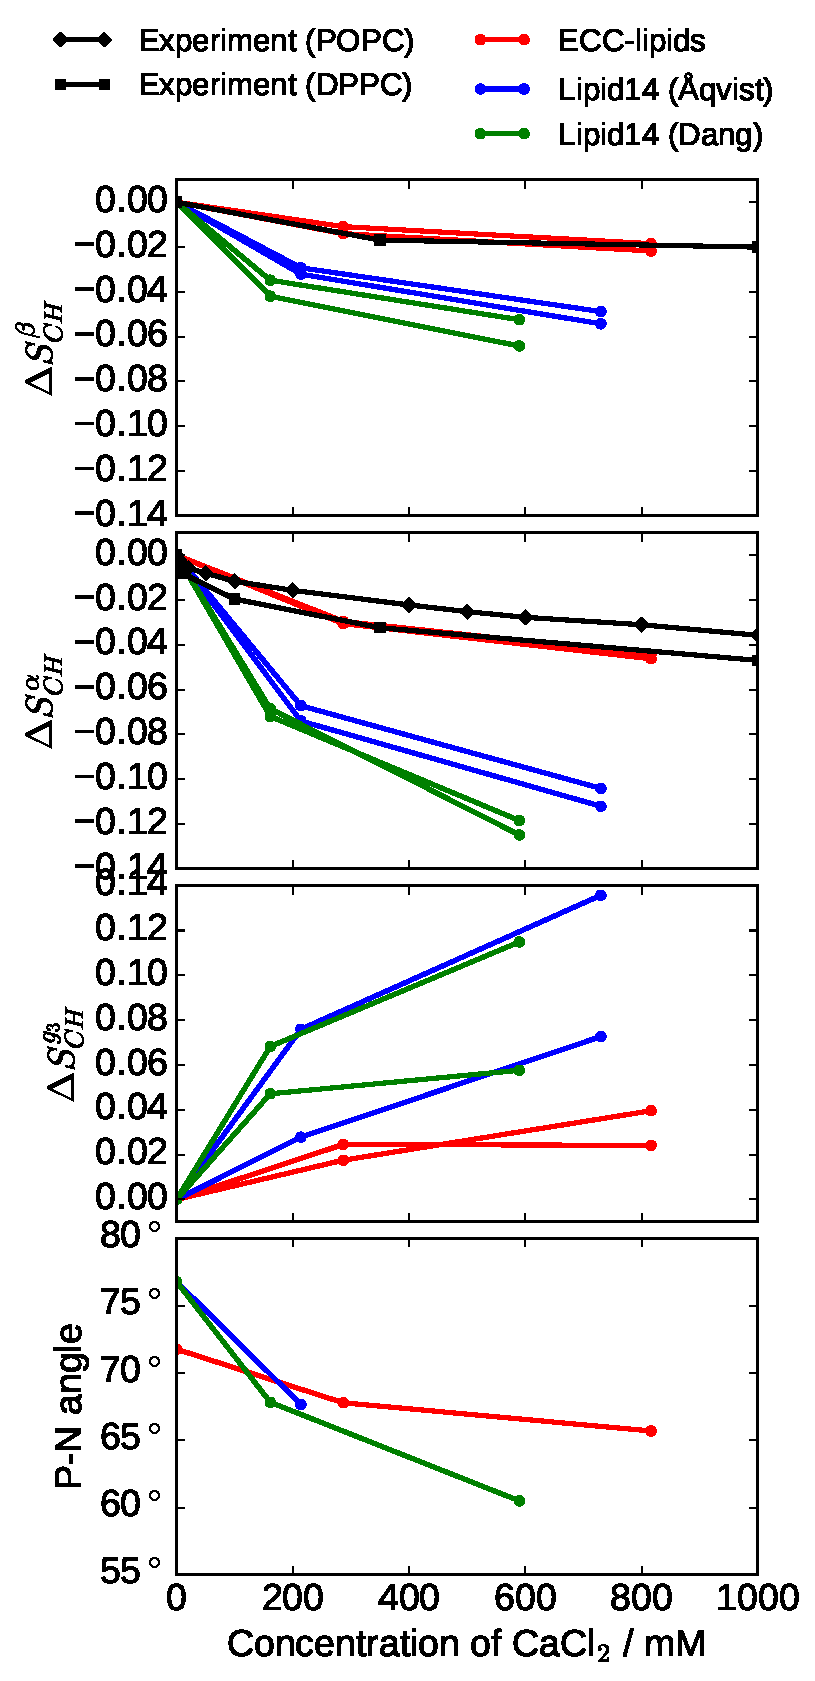
\includegraphics[width=8.0cm]{../Fig/ipython_nb/PN_angle_OrdPars-A-B-g3_L14-ECCL17_q80_sig89_CaCl.pdf}
  \caption{\label{fig:delta_ordPar_CaCl}
    Changes of the head group order parameters and P-N vector orientation of a POPC bilayer 
    as a function of the CaCl$_2$ concentration
    are shown from simulations with different force fields together with experimental data 
    (DPPC (323\,K) \cite{akutsu81} and POPC (313\,K) \cite{altenbach84}). 
    Ion concentrations in bulk water are shown in x-axis. 
    Bulk concentrations from simulations are calculated 
    from the farthest point from the lipid bilayer in the aqueous phase
    with an error estimate of 10\,mM.
    The error estimate for the simulation with Lipid14 and ECC-ions is an order of magnitude larger, 
    because the simulation cell was too small (shown if Fig.~\ref{fig:cacl-dens}). 
    Simulation data with Lipid14 and \AA{}qvist ion parameters are taken directly from
    Refs.~\cite{lipid14POPC0mMNaClfiles,lipid14POPC350mMCaClfiles,lipid14POPC350mMCaClfilesNC}.
  }
  %\todo{Experimental values from \cite{akutsu81} to be put in the $g_3$ figure:
    %the value of $g_3$ order parameter of DPPC was -0.214 
    %in the absence of ions [average of two closely spaced splittings] and -0.211 in the presence
    %of 0.35 M CaCl$_2$ (at 59 Celcius). No effect of ions could be detected on DPPC bilayers labeled
    %at the C-2 segments of both fatty acyl chains.'' }
\end{figure}

\begin{figure}[htb!]
  \centering
  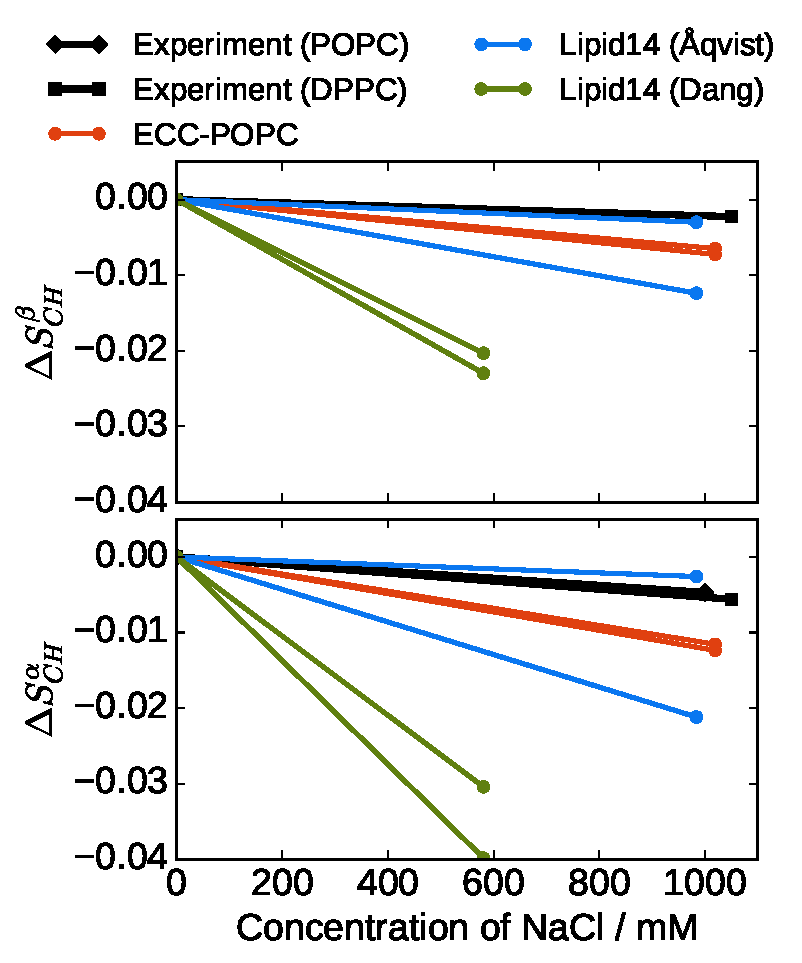
\includegraphics[width=8.0cm]{../Fig/ipython_nb/OrdPars-A-B_L14-ECCL17_q80_sig89_NaCl.pdf}
  \caption{\label{fig:delta_ordPar_NaCl}
    The changes of the head group order parameters of a POPC bilayer as a function of NaCl concentration
    from simulations with different force fields together with 
    experimental data for DPPC (323\,K) \cite{akutsu81} and POPC (313\,K) \cite{altenbach84}.
    Ion concentrations in x-axis are calculated as in Fig.~\ref{fig:delta_ordPar_CaCl}.
    Simulation data with Lipid14 and \AA{}qvist ion parameters are taken directly from
    Refs.~\cite{lipid14POPC0mMNaClfiles,lipid14POPC1000mMNaClfiles}.
  }
  %\todo{Add also the POPC result to the figure. Ref.\cite{altenbach84} gives for POPC at 1M of NaCl $\Delta S^\alpha=(6.1-5.5)*0.00784=0.004704$.} \\
\end{figure}


Changes of the lipid bilayer headgroup order parameters from different simulations and
experiments \cite{akutsu81,altenbach84} are shown in Figs.~\ref{fig:delta_ordPar_CaCl} and~\ref{fig:delta_ordPar_NaCl}
as functions of NaCl or CaCl$_2$ concentrations.
%Responses to NaCl concentrations are in SI, Fig.~S\ref{fig:delta_ordPar_NaCl}.
These results can be used to compare the ion binding affinities to lipid bilayers
between simulations and experiments using the electrometer concept, because 
the order parameters decrease proportionally 
to the amount of the bound positive charge (Fig.~\ref{OrderParameterCHANGESsurf} and Ref.~\citenum{seelig87,catte16}). 
A recent comparison of different simulation models to the experimental data
revealed that most force fields significantly overestimate Na$^+$ ion binding to PC
lipid bilayers and that none of the available models correctly reproduces
the details of the binding of Ca$^{2+}$ ions \cite{catte16}.
The only exception in Ref.~\citenum{catte16} was the Lipid14 model \cite{dickson14} simulated with \AA{}qvist ions,
which reproduced the experimentally measured 
small order parameter changes with NaCl (Fig.~\ref{fig:delta_ordPar_NaCl})
and the negligible Na$^+$ binding to PC bilayers \cite{akutsu81,altenbach84}.
However, the change of the headgroup order parameters as a function of CaCl$_2$ concentration 
(Fig.~\ref{fig:delta_ordPar_CaCl}) was still grosly overestimated within this model.

Since artifacts were reported in simulations with \AA{}qvist ions is water \cite{auffinger07},
we also simulated the Lipid14 model with more realistic ion models by Dang et al.~\cite{smith94,chang1999,dang2006}, and
ECC-ions~\cite{jungwirth17-new-paper-to-be-published, Pluharova2014}. 
However, we still observed overestimated binding for both \ce{Ca^{2+}} and Na$^+$ with these ions models 
(Figs.~\ref{fig:delta_ordPar_CaCl} and~\ref{fig:delta_ordPar_NaCl}). 
The results are in line with the previous work \cite{catte16},
suggesting that additional improvements in the lipid parameters are
required to correctly describe the binding of cations to phospholipid bilayers.

%To improve the cation binding behaviour to POPC lipid bilayer we implicitly included the electronic
%polarization to the Lipid14 model by using the ECC approach as described in section \ref{section:ecc}.
The results from the simulations combining the ECC-lipids with the ECC-ion models \cite{jungwirth17-new-paper-to-be-published, kohagen16, Pluharova2014}
exhibit a significanlty improved behavior of cation binding to the POPC bilayer in Fig.~\ref{fig:delta_ordPar_CaCl},
showing a good agreement with experiments in the changes of 
the lipid headgroup order parameters as functions of NaCl or CaCl$_2$ concentrations.
Since also the headgroup order parameter
response of the ECC-lipids model the to the bound positive charge 
is in good agreement with experiment (see above section \ref{section:boundCHARGE}),
we can conclude that this model correctly reproduces the binding affinities of
Na$^{+}$ and Ca$^{2+}$ ions to the POPC lipid bilayer.

In addition, while the response of the glycerol backbone $g_3$ order parameter to CaCl$_2$ was
signifincantly overestimated in the original Lipid14 model, the ECC-lipids model
provides a greatly improved agreement with experiment, as seen in Fig.~\ref{fig:delta_ordPar_CaCl}.
Also the changes of the P-N vector angle are too pronounced
for the Lipid14 model, for which the largest tilting toward water phase 
induced by a $780\,\mathrm{mM}$ CaCl$_2$ concentration
is approximately 17$^{\circ}$, while the corresponding
value for ECC-lipids model is only 6$^{\circ}$ ($820\,\mathrm{mM}$ CaCl$_2$).

Within the Lipid14 model, 
the overestimated changes in the lipid headgroup order parameter of POPC  as functions of the CaCl$_2$ concentration arise both from the overestimated
binding affinity and the too strong sensitivity of the headgroup tilt to the bound positive charge.
This likely applies also to the other lipid models tested in a previous study~\cite{catte16},
which underlines the importance of the comparison of the lipid headgroup order parameter response
to the bound charge between simulations and experiments as presented in section \ref{section:boundCHARGE}.

Finally, the ion binding affinities for the ECC-lipids model with different water models are compared in SI. 
In general, the performance of ECC-lipids with any of the water models 
is better than that of the original Lipid14 model, with the order parameter changes being slightly overestimated
with the four-site water models and with TIP3p model.


%\todo{SAMULI: Maybe we should discuss the repeat distances and
%  area per molecules measured at \cite{petrache06,pabst07,uhrikova08}
%  }





\subsection{Structure and affinity of cation binding to POPC membrane}
\label{sec:affinity}

\begin{table}[tb!]
  \caption{Relative surface excess of calcium with respect to water, 
  and the ratios of the amount of calcium cations 
  bound to phosphate or carbonyl moieties 
  to the amount of such cations bound to both moieties in a POPC bilayer 
  from various simulation models. 
  $C_w$ is the concentration of CaCl$_2$ in water before adsorbing to the phospholipid bilayer. 
  \label{tab:binding}}
  \begin{tabular}{l|c | c c | c c}
    model                 & $\Gamma_{Ca}^w \,/\, \mathrm{nm}^{-2}$ & $C_{w}$ & $C_b\,/\,\mathrm{mM}$   & $r^\mathrm{Ca^{2+}} _\mathrm{PO_4} $ & $r^\mathrm{Ca^{2+}} _\mathrm{O_{carb.}} $ \\
    \hline
    ECC-lipids            &  $0.06 \pm 0.01 $ &  350  &  $280\pm 10 $  &  99\%  &    25\%    \\
    Lipid14/\AA{}qvist    &  $0.13 \pm 0.01 $ &  350  &  $210\pm 10 $  & 100\%  &    37\%     \\
    Lipid14/Dang          &  $0.23 \pm 0.03 $ &  350  &  $160\pm 10 $  & 100\%  &    14\%    \\
    Lipid14/ECC-ions      &  $0.35 \pm 0.11 $ &  350  &  $120\pm 100$  & 100\%  &    23\%    \\
%Average no. of bound cations:
%L14+Aqvist: all:22.7, phos:22.7, carb:8.5
%L14+Dang:   all:29.2, phos:29.2, carb:4.0
%L14+ECC-ion:all:37.7, phos:37.7, carb:8.5
  \end{tabular}
\end{table}

Binding affinities of Ca$^{2+}$ ions to a POPC bilayer in different simulation 
models were quantified by calculating the relative surface excess of calcium with respect to water molecules, $\Gamma_{\rm Ca}^w$, from Eq.~\ref{surfexcess}.
%using the bulk concentrations determined from the density profiles in Fig.~\ref{fig:cacl-dens}. 
The values of $\Gamma_{\rm Ca}^w$, shown in Table~\ref{tab:binding},
were calculated from simulations with the same concentration of CaCl$_2$ of $350\,\mathrm{mM}$  with 
respect to water before solvating the lipids.
As expected from the changes of the lipid headgroup order parameters in Fig. \ref{fig:delta_ordPar_CaCl}, 
the relative surface excess for the ECC-lipids model, $\Gamma_{\rm Ca}^w = (0.06 \pm 0.01) \rm{nm}^{-2}$,
is significantly smaller than for the Lipid14 model with \AA{}qvist ions, $\Gamma_{\rm Ca}^w = (0.13 \pm 0.01) \rm{nm}^{-2}$,
or with Dang ions, $\Gamma_{\rm Ca}^w = (0.23 \pm 0.03) \rm{nm}^{-2}$,
or with ECC-ions,  $\Gamma_{\rm Ca}^w (0.35 \pm 0.11) \rm{nm}^{-2}$,
where the large uncertainity arises from a too small simulation box (Fig.~\ref{fig:cacl-dens}).
Interestingly, the relative surface excess of 
\ce{NaCl} at $1\,\mathrm{M}$ concentration (ECC-ions~\cite{Pluharova2014}) 
%calculated using density profiles in Fig.~\ref{fig:cacl-dens}
is not only quantitatively but also qualitatively different from \ce{CaCl2}
having a negative value $\Gamma_i^w = (-0.11 \pm 0.01) \rm{nm}^{-2}$ 
meaning that water molecules are preferred to sodium and chloride ions at the membrane-water interface. 
This is in contrast to the most of the available lipid force fields,
which predict a positive binding of sodium to
PC lipid bilayers \cite{catte16}.
%\todo{JOE: Add references to NaCl simulation papers that show peaks.
%Add a simple note that there is NBFIX trick in Charmm36 (?).} 
%SAMULI: I think that it is enough to cite NMRlipids II here, which shows all the results
%
%This finding is depicted in Figures~\ref{fig:nacl-dens} and~\ref{fig:cacl-dens},
%which show the density profile of ions and water along the membrane normal. 
%
%The density profiles show
%a larger Ca$^{2+}$ density peak in lipid headgroup region for
%the Lipid14 model with Dang and ECC-ions than for the ECC-lipids model.


\begin{figure}[htbp!]
  \centering
  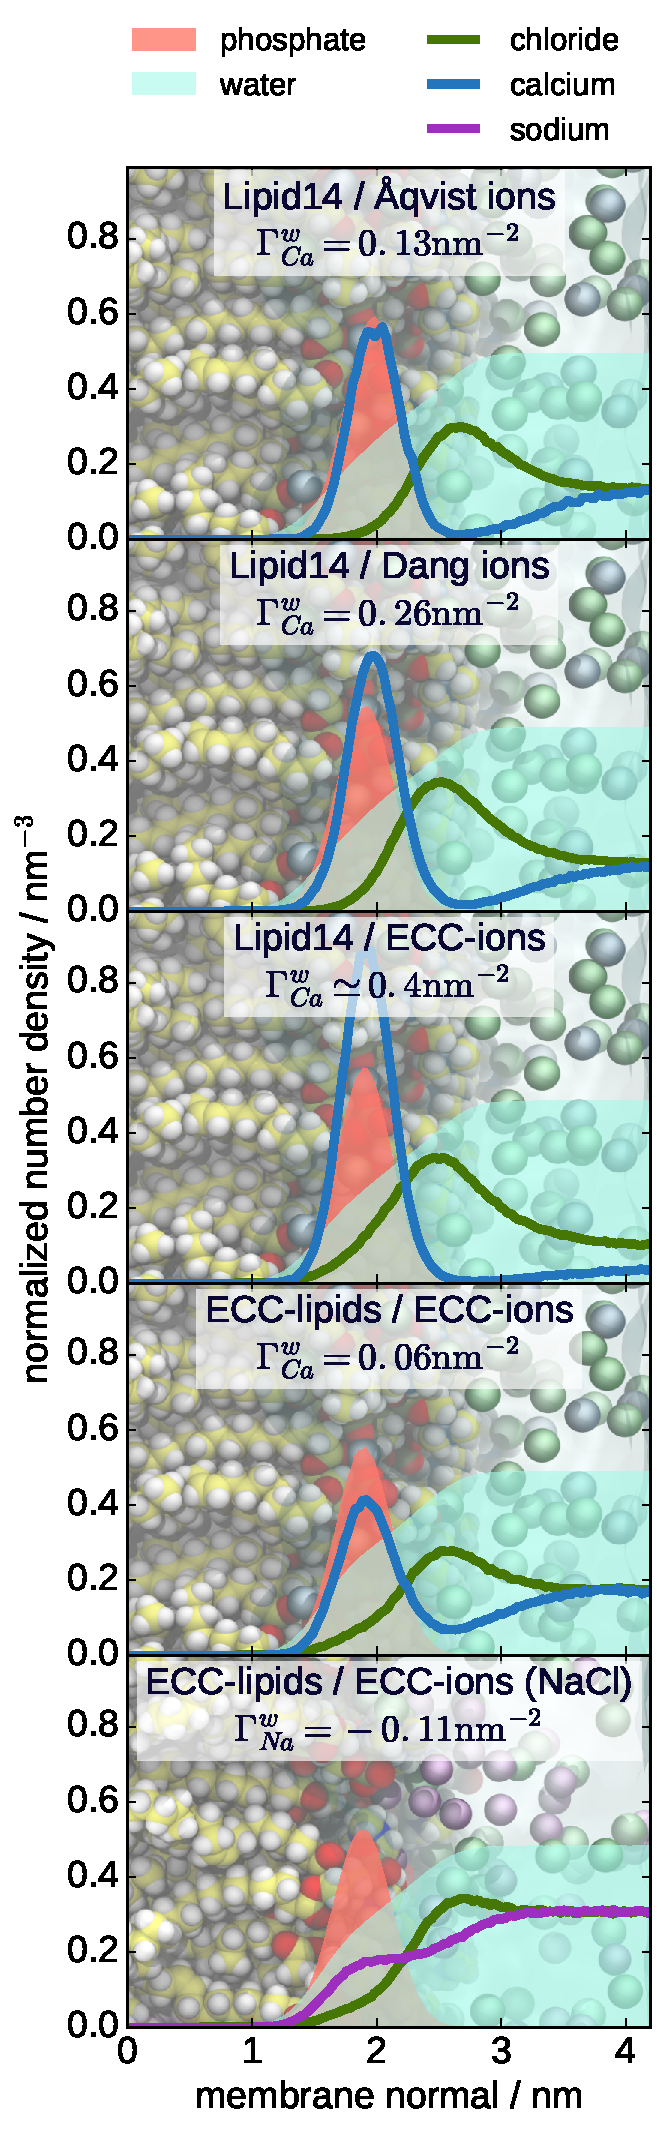
\includegraphics[height=19.5cm]{../Fig/ipython_nb/density_profiles_ca_cl_wat_phos_models-compar.pdf}
  \caption{\label{fig:cacl-dens}
    Number density profiles of \ce{Ca^{2+}}, \ce{Na^{+}} and \ce{Cl^-} along membrane normal axis
    for different force fields. Data for Lipid14 with \AA{}qvist ions are taken directly from Ref. \citenum{catte16}.
    %Normalization factor for ions is 1 for monovalent ions (i.e.~\ce{Na^+} and~\ce{Cl^-}),
    In order to visualize the density profiles with a scale comparable to the profile of \ce{Ca^{2+}}, 
    densities of~\ce{Cl^-} and \ce{Na^{+}} are divided by 2, and
    densities of phosphate group resp. water are divided by 5 resp. 200. 
    The molar concentration of ions in water is 350~mM in all systems
    presented here. 
    }
\end{figure}

In a POPC bilayer, the ratio of the amount of calcium cations 
bound to either phosphate or carbonyl moieties 
to the amount of such cations bound to both moieties
from various simulation models
%The probabilities for a bound \ce{Ca^{2+}} ion to interact with
%different oxygen moieties of POPC 
%$\Sigma ^\mathrm{Ca^{2+}} _\mathrm{O}$,
was analyzed by counting the contacts within the distance of $0.3 \, \mathrm{nm}$, 
as done previously in Ref.~\citenum{javanainen17}. 
%
%SAMULI: I commented out the average number of contacts. All the essential information
%for this is in the probabilities.
%
%In contrast to sodium, the dominant contribution
%to the binding of \ce{Ca^{2+}} to POPC membranes comes from the phosphate group. 
%% Numbers from simulation with 346mM conc. CaCl2 (OPC3)
%The average number of contacts per lipid 
%between \ce{Ca^{2+}} at $290\,\mathrm{mM}$ concentration and any oxygen atom in POPC is 
%$\Sigma ^\mathrm{Ca^{2+}} _\mathrm{O} = 0.134 $,    % = 17.1/128 
%whereas if only phosphate oxygen atoms are considered 
%the average number of contacts decreases only by a tiny amount to 
%$\Sigma ^\mathrm{Ca^{2+}} _\mathrm{PO_4} = 0.133 $,    % = 17.0/128 . 
%and if only carbonyl oxygen atoms are considered 
%%(phosphate oxygens contribute, but are not counted as contacts),
%this value is merely
%$\Sigma ^\mathrm{Ca^{2+}} _\mathrm{O_{carb.}} = 0.033 $.    % = 4.3/128 . 
%
% Numbers from simulation with 980/845mM conc. CaCl2 (OPC3)
%The average number of contacts per lipid between \ce{Ca^{2+}} and any oxygen atom in POPC is 
%$\Sigma ^\mathrm{Ca^{2+}} _\mathrm{O} = 0.264 $,    % = 33.8/128 
%whereas if only phosphate oxygen atoms are considered 
%the average number of contacts decreases only by a tiny amount to 
%$\Sigma ^\mathrm{Ca^{2+}} _\mathrm{PO_4} = 0.262 $,    % = 33.5/128 . 
%and if only carbonyl oxygen atoms are considered 
%(phosphate oxygens contribute, but are not counted as contacts),
%this value is merely
%$\Sigma ^\mathrm{Ca^{2+}} _\mathrm{O_{carb.}} = 0.066 $.    % = 8.4/128 . 
The results in Table \ref{tab:binding} show that almost all (99\%) of the 
bound Ca$^{2+}$ ions are in contact with the phosphate oxygens,
with two thirds (67\%) interacting only with these species,
while the remaining one third (32\%), interacting also with the carbonyl oxygens. 
The interactions between
calcium ions with only carbonyl oxygens are very unlikely (1\%).
The individual lipids or acyl chains were not distinguished in the analysis,
hence, simultaneous contacts of ions with both oxygen moieties may be inter or intra molecular,
and may occur with carbonyls in either of the acyl chains.
The most likely interactions between Ca$^{2+}$ ions and phosphate oxygens are visualized with
the probability density isocontours in Fig.~\ref{fig:volmaps}.
While the higher concentrations of \ce{CaCl2} naturally increases the amount of contacts per lipid,
%for $850\,\mathrm{mM}$ concentration of \ce{CaCl2}
%the average number of contacts per lipid is increased to
%$\Sigma ^\mathrm{Ca^{2+}} _\mathrm{O} = 0.264 $, 
the distribution of contacts between phosphate and carbonyl oxygens is not affected.
%and density profiles of ions and water along the membrane normal in Fig.~\ref{fig:cacl-dens}. 

\begin{figure}[tb!]
  \centering
  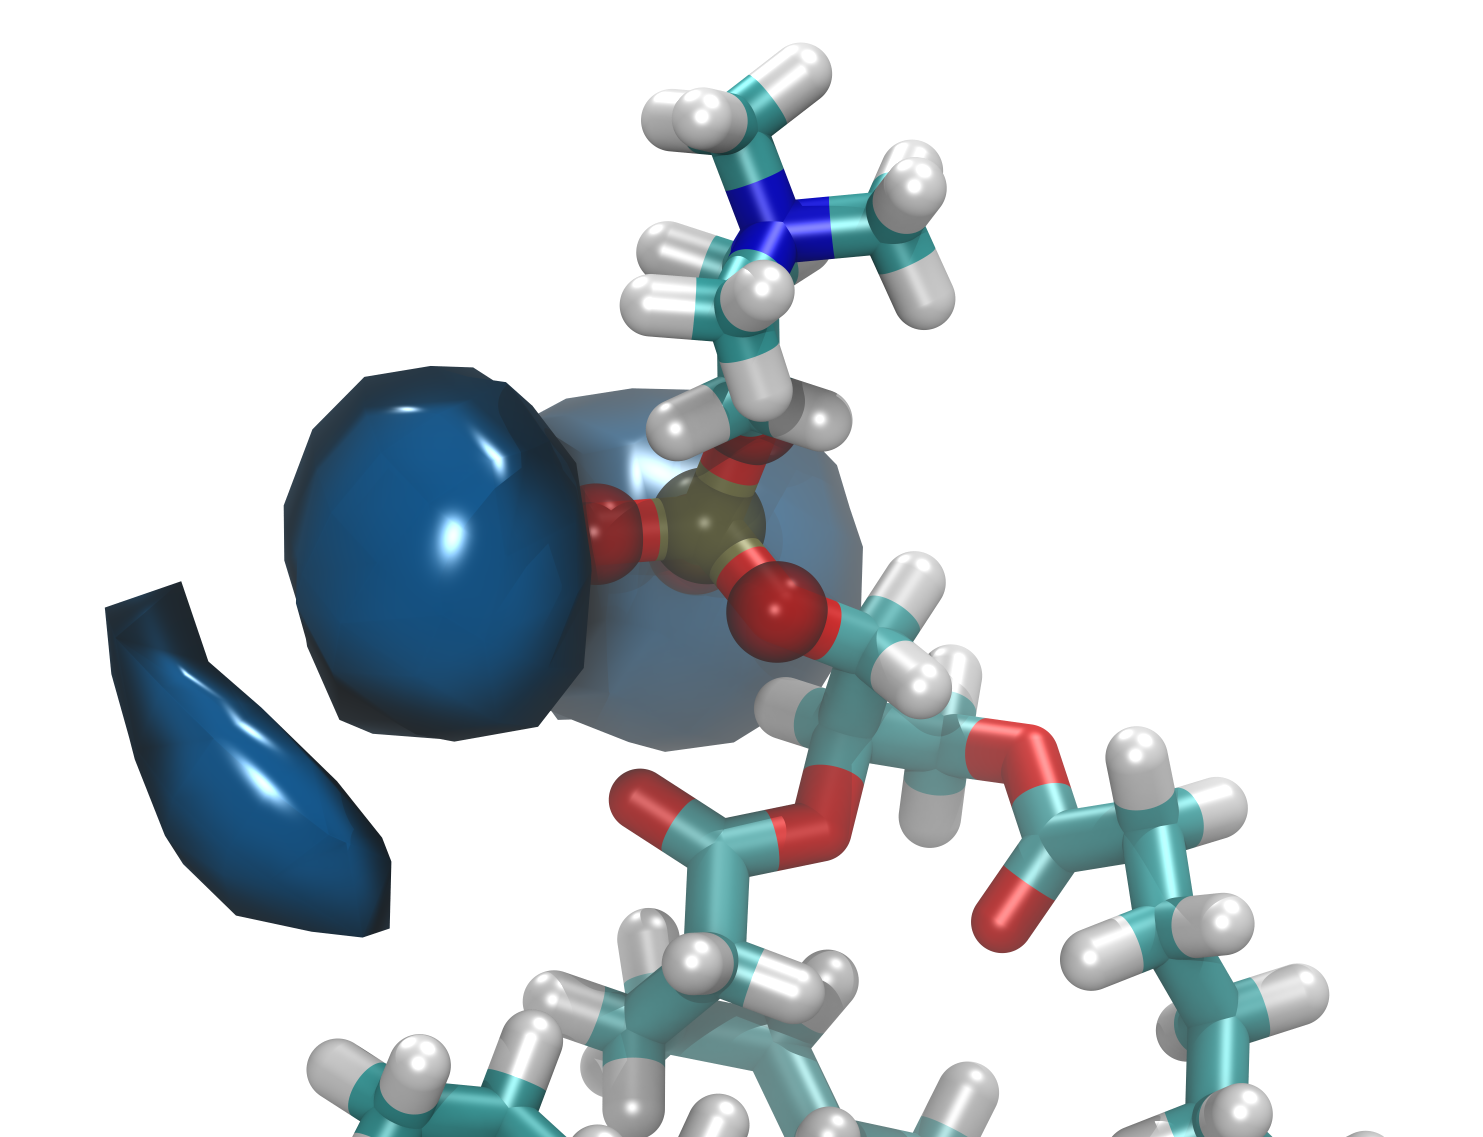
\includegraphics[width=8.0cm]{../Fig/volmap_resid10_Ca_Cl_PO4Cent.png} %\\
%  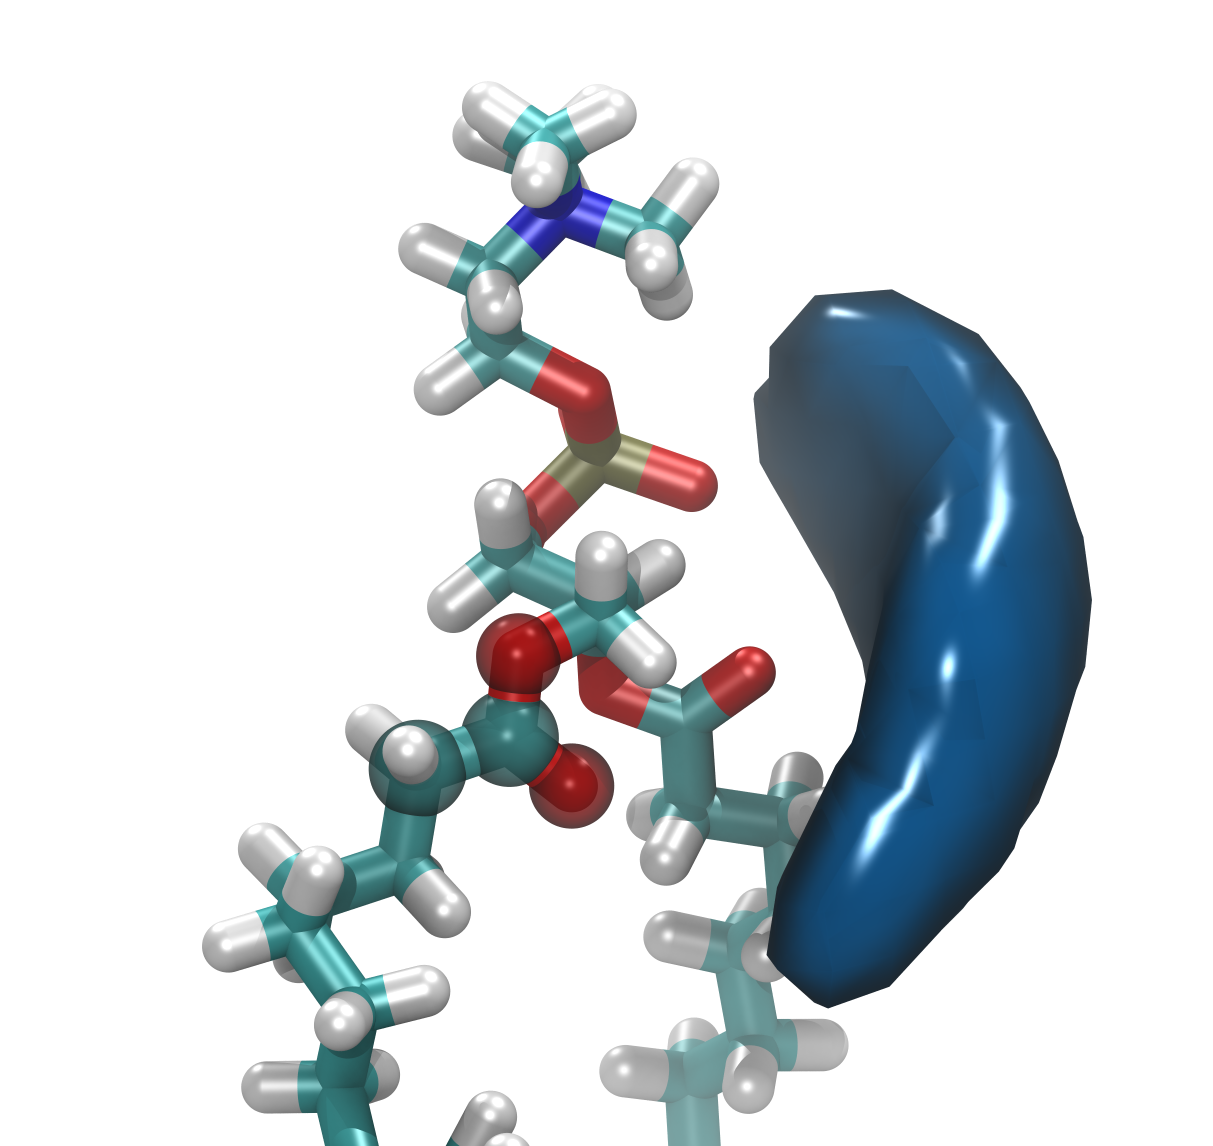
\includegraphics[width=4.0cm]{../Fig/volmap_resid10_Ca_Cl_sn1Cent.png}
%  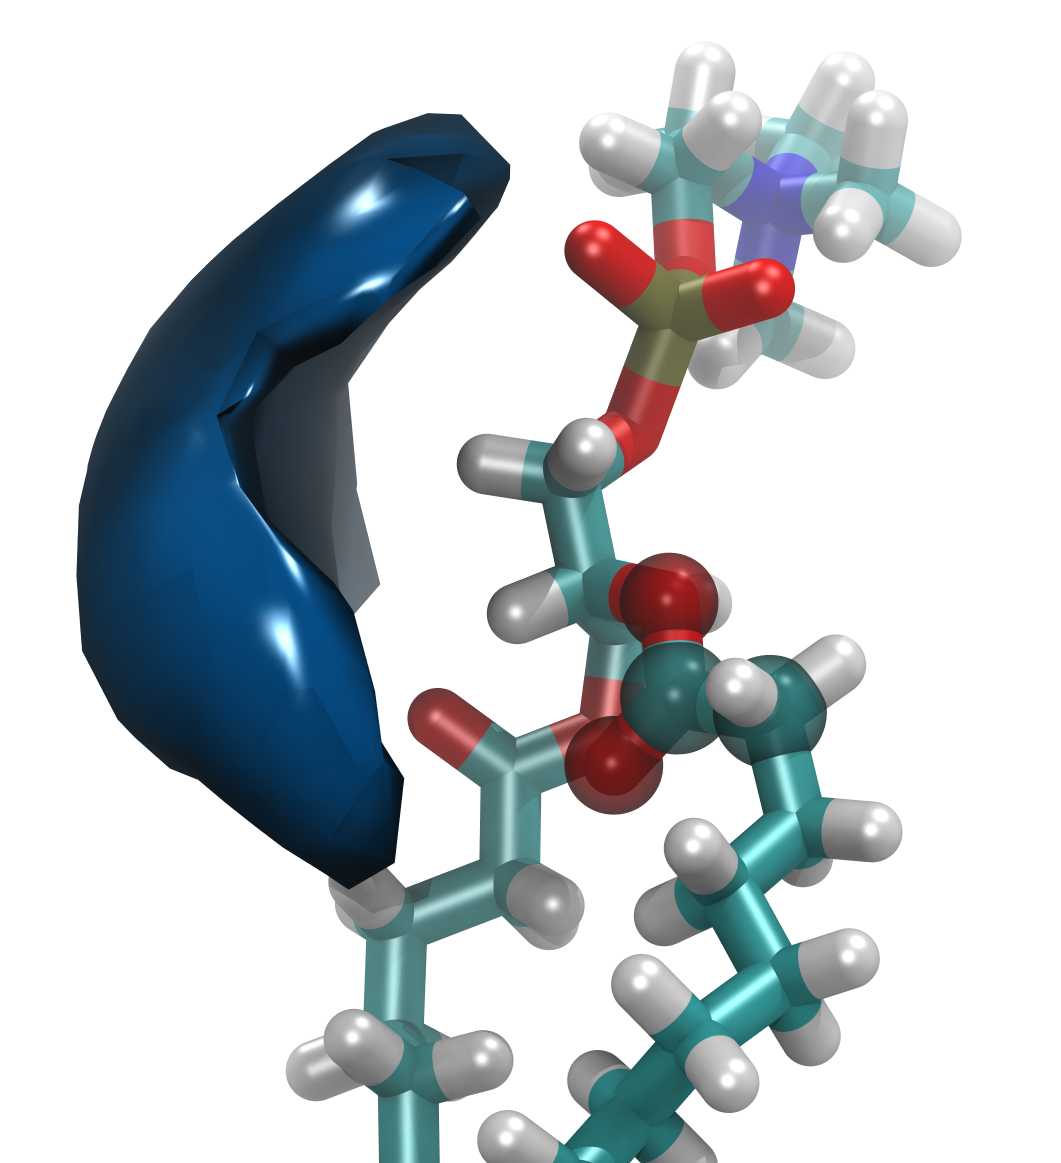
\includegraphics[width=3.6cm]{../Fig/volmap_resid10_Ca_Cl_sn2Cent.png}
  \caption{\label{fig:volmaps}
      Isocontours of probability density of \ce{Ca^{2+}} with respect to 
      the phosphate oxygens of POPC from ECC-lipids simulation.
      The probability density was evaluated around a single lipid, 
      after its strucutral alignment using only phosphate group. 
      %moiety, side chain 1 carbonyl group and side chain 2 carbonyl group.
      %Shown contours suggest that the dominant contribution 
      %to \ce{Ca^{2+}} binding comes from the phosphate oxygens,
      %whereas the interactions with any of the two carbonyl groups are considerably milder.
  }
  \todo{JOE: I'll update this figure with some ensemble of configuration to support binding preference of \ce{Ca^{2+}}
  SAMULI: I am not sure if this would be needed anymore.}
\end{figure}

Even though \ce{Na+} ions do not specifically bind to a POPC bilayer,
they still interact with its oxygen moieties. 
%the average number of contacts per lipid with any oxygen atom in POPC is 
%$\Sigma ^\mathrm{Na^{+}} _\mathrm{O} = 0.106 $,    % = 17.1/128 
%whereas if only phosphate oxygen atoms are considered 
%this number decreases to 
%$\Sigma ^\mathrm{Na^{+}} _\mathrm{PO_4} = 0.085 $,    % = 17.0/128 . 
%and if only carbonyl oxygen atoms are counted 
%it is even lower, 
%$\Sigma ^\mathrm{Na^{+}} _\mathrm{O_{carb.}} = 0.048 $.    % = 4.3/128 . 
The results  from simulation at $1\,$M \ce{NaCl} concentration show 
that 55\% of \ce{Na+} ions interact with only phosphate oxygens of POPC 
and 20\% with only carbonyl oxygens,
and the rest, 25\%, is interacting with both.
%, phosphate and carbonyl oxygens.  
%This is in line with the calculated negative value of 
%relative surface excess of sodium with respect to water, $\Gamma_i^w$, and
%their density profiles along the membrane normal (Fig.~\ref{fig:nacl-dens})
%suggesting that the populations of bound sodium cations 
%naturally decrease with the decreasing density of water. 

In conclusion, the results suggest that calcium ions bind specifically to phosphate
oxygens, occasionally interacting also with carbonyls. This is in good agreement
with previous conclusions from several experimental and computational
studies~\cite{hauser76,hauser78,herbette84,cevc90,binder02}, but
suggesting a lower relative binding affinity to the carbonyls than inferred from previous MD simulation
studies~\cite{bockmann03,bockmann04,melcrova16,javanainen17}.
Sodium ions also interact primarily with phosphate oxygens of the POPC, 
but in contrast to calcium, the interactions purely with carbonyls are also significant.
The physiological relevance of these details of sodium interactions is, however, unclear
due to its overall very weak binding affinity.

\subsection{Binding stoichiometry of \ce{Na+} and \ce{Ca^{2+}} cations to the POPC membrane}

%Binding probability:
%\ce{Ca2+} complex with \\
%1 POPC - 13\% -- 30\% \\
%2 POPC - 18\% -- 42\% \\
%3 POPC - 12\% -- 28\% \\

Simple binding models have been used previously to interpret
the same experimental data \cite{altenbach84,macdonald87} 
that are used in this work to validate the simulation models in Fig. \ref{fig:delta_ordPar_CaCl}.
Results from measurements of the lipid headgroup order parameters and from
atomic absorption spectroscopy were best
explained by a ternary complex binding model with a binding
stoichiometry of one \ce{Ca^{2+}} per two POPC lipids~\cite{altenbach84}.
However, a Langmuir adsorption model (i.e. \ce{Ca^{2+}}:POPC stoichiometry of 1:1) 
also provided a good fit to the experimental data when only low concentrations of \ce{CaCl2} were considered~\cite{macdonald87}.
Note that the results based on these binding models and the measured headgroup order parameter changes
are also inluded in the tabulated experimental binding constants~\cite{marsh13}.

Since the same experimental data are reproduced by the present ECC-lipids model,
we can use the model to provide a more detailed interepration of the binding stoichiometry than
the previously used simple binding models~\cite{altenbach84,macdonald87}. To directly evaluate the
stoichiometry from simulations we calculated the relative propensities of \ce{Ca^{2+}}:POPC
complexes with various stoichiometries by counting the individual lipid
molecules within the distance $0.3\,\mathrm{nm}$ from each \ce{Ca^{2+}} ion,
as already done in the previous section~\ref{sec:affinity}.
The results from POPC simulation with a 285~mM concetration of CaCl$_2$ in
Fig.~\ref{fig:cacl_complexes} demonstrate the largest propensity (41\%) for the
ternary complex with the \ce{Ca^{2+}}:POPC stoichiometry of 1:2, but 
the probabilities of complexes with the stoichimetries of 1:1~(25\%)~and
1:3~(34\%)~are only slightly lower. This
suggests a more complex binding model than the previous simple ternary complex model.
%The observed propensities of
%$41\%$ for two lipids,
%$25\%$ for one lipid, and
%$34\%$ for three lipids 
With a broad brushstroke, the simulation data can, however, be viewed such that
one calcium binds to two lipids on average,
because the probabilities of the complexes with 1 or 3 lipids are almost equal to each other 
(and complexes with more than three lipids per one calcium ion were not observed).  
This probably explains why the simple the ternary complex model fits the
experimental data, as well as the ECC-lipids simulation results, rather well
(see Fig.~S\ref{fig:cacl-bind} in SI and its caption for details). 


\begin{figure}[tb!]
  \centering
  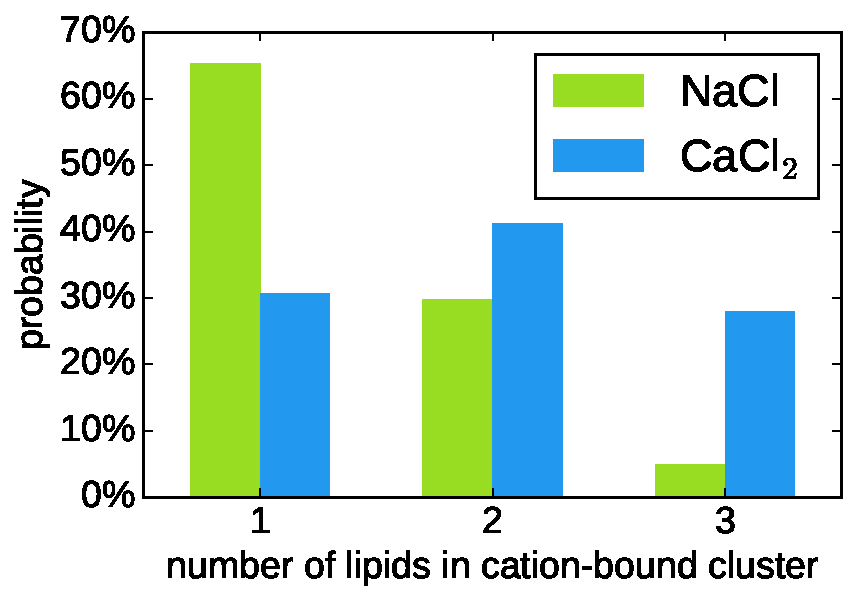
\includegraphics[width=8.0cm]{../Fig/ipython_nb/stoichiometry_NaCl-CaCl2_comparison_Ecc-lipids.pdf} \\
  \caption{\label{fig:cacl_complexes}
      Relative probabilities of existence of \ce{Na^{+}} or \ce{Ca^{2+}} complexes
      with a certain number of POPC lipids. 
      \ce{Na^{+}} complexes were evaluated from the simulation with 1~M concentration;
      and \ce{Ca^{2+}} complexes were evaluated from the simulation with 287~mM concentration.
  }
\end{figure}

The probabilities of different complexes formed by \ce{Na+} ions and POPC
analyzed from the simulation with the ECC-lipids model at $1\,$M concentration of NaCl are also 
shown in Fig.~\ref{fig:cacl_complexes}. In contrast to calcium, the
probability is largest (67\%) for 1:1 complex, significantly smaller (29\%)
for 1:2 complexes and very small (4\%) for 1:3 of \ce{Na+}:POPC complexes.




\subsection{Residence times of \ce{Na+} and \ce{Ca^{2+}} cations in POPC membrane}

Equilibration of \ce{Ca^{2+}} ions at the POPC bilayer takes hundreds of
nanoseconds in MD simulations with current state of the art force fields,
e.g. CHARMM36 and Slipids force fields~\cite{javanainen17}, suggesting that
simulations at a temporal scale of several microseconds are required
to reach the binding/unbinding equilibrium. 
This is in line with the density profiles of \ce{Ca^{2+}} 
from simulations in Fig.~\ref{fig:cacl-dens}, 
which all show a region of a very small calcium density 
around the level of cholines in POPC (i.e. around $2.5\,\mathrm{nm}$).
In contrast, simulations with  ECC-lipids 
exhibits only a relatively shallow local
minimum at that level.
This suggests that the smaller barrier for the exchange of calcium ions 
shall lead to their faster exchange with the solvent within ECC-lipids.
To quantify the exchange of ions between the membrane and solvent in simulations, we thus calculated 
residence times of ions bound to the membrane.
We use the same definition for ions bound to the membrane as in the above section~\ref{sec:affinity},
i.e., an ion is considered as bound if it is within 0.3~nm from any oxygen atom
belonging to a lipid molecule in a bilayer.

The histograms of residence times of \ce{Ca^{2+}} in a POPC bilayer 
at a $450\,\mathrm{mM}$ concentration of \ce{CaCl_2} in water before adsorption to phospholipids
from simulations with ECC-lipids 
compared to CHARMM36 (taken from previous study \cite{javanainen17}, 
simulation data available at Ref.~\citenum{zenodo.259376})
are shown in Fig.~S\ref{fig:hist_residence_times} in SI. 
%Based on Fig. S17 in that work, Ref.~\citenum{javanainen17},
%we took the simulation with the apparent highest fluctuations of the number of bound calcium,
%which can be obtained at \url{https://doi.org/10.5281/zenodo.259376}
%and anaylsed the residence times.
In the CHARMM36 simulation, approximately 20\% of the \ce{Ca^{2+}} residence times are longer than
the whole length of the trajectory ($800\,\mathrm{ns}$).
Within such a relatively short simulation, 
we can only estimate that 
less than 60\% of the bound residence times 
is due to cations interacting with the phospholipid membrane 
for less then half of the simulation length~(400~ns).
Even longer residence times are observed
in  simulations with CHARMM36 and Slipids models reported in previous works~\cite{javanainen17}.

In contrast, at least an order of magnitude faster bound/unbound calcium exchange is observed within the
ECC-lipids model, where 90\% of the \ce{Ca^{2+}} residence times to a POPC membrane are 
shorter than $60\,\mathrm{ns}$, % exactly $53\,\mathrm{ns}$.
The longest observed residence time is now $141\,\mathrm{ns}$, 
which is well below the total length of the simulation used for analysis, i.e., 200~ns.
The exchange of \ce{Na+} ions at the POPC membrane is
another order of magnitude faster, yielding 90\%
of the residence times smaller than~$1\,\mathrm{ns}$, with
the longest residence time being~$6\,\mathrm{ns}$. 
\todo{Joe: the following is a bit more subtle argument. 
I deem it not necessary to include it in the paper, however, 
the experimental estimate of less tan 10us holds likely also for Charmm36/ECC-ions, as stated before.}
Note that the ECC-lipids calcium results are in line with the experimental estimate that 
the residence time of \ce{Ca^{2+}} at each individual PC headgroup 
is shorter than $10\,\mu\mathrm{s}$~\cite{altenbach84}.

%give a roughly estimate of the order
%of $1\,\mu\mathrm{s}$
%This is unfortunately not the case of many theoretical works,
%where the residence time cannot be estimated,
%or the simulation has not even decorrelated from it's 
%initial condition with a population of bound/unbound cations \cite{catte16}, 
%because it is limited by the simulation length, 
%even though it can be very long (order of $\mu\mathrm{s}$) in some works, e.g. reference~\citenum{javanainen17}. 
%Increasing time scales to the order of $\mu\mathrm{s}$ 
%doesn't help to alleviate such a problem in current lipid models \cite{javanainen17}. %and also \cite{catte16}, but same simulation was used. 

In conclusion, the results from the ECC-lipids model suggest that the
exchange of calcium between the POPC bilayer and the solvent occurs within $\sim 100\,$ns timeframe,
which is significantly faster than previously reported~\cite{javanainen17}.
Sodium cations exhibit an even a faster exchange.
This all suggests that simulations with a length of a several hundreds of
nanoseconds are sufficient to simulate ion binding
to phospholipid bilayers in equilibrium, when realistic force fields are used.
This has not been the case with previous lipid force fields,
which overestimate the binding strength of the sodium and calcium cations \cite{javanainen17,catte16}.
%Such a finding changes the point of view on binding of calcium to PC membranes from
%a very strong long-term stable binding with rare exchanges to 
%a relatively frequent exchange of clacium cations 
%in equilibrium between membrane and solvent. 








\section{Conclusions}

In this study, we employed the electrometer concept to demonstrate that the binding of \ce{Na^+} and \ce{Ca^2+} ions
to a POPC lipid bilayer can be accurately described within a classical MD simulation 
force field, provided that electronic polarization is implicitly included via 
the electronic continuum correction~\cite{leontyev11}.
While the structural details of a POPC lipid bilayer simulated with the newly developed ECC-lipids
model agree with experiments with an accuracy comparable to the other state of the art lipid models,
the model also reproduces the experimental lipid head group order parameter responses to
a cationic surfactant, NaCl and CaCl$_2$ concentrations. 
It thus represents a significant improvement over 
other available lipid models, which overestimate cation binding affinities~\cite{catte16}.  
The ECC-lipids model is build upon
the Lipid14 POPC model~\cite{dickson14} by scaling the partial charges by a factor of 0.8
and reducing the Van der Waals radii by a factor of 0.89 for the headgroup, glycerol backbone and carbonyl atoms. 

The good agreement with experiments enables us to 
interpret NMR experiments with atomistic details using MD simulations with the ECC-lipid model.
In line with previous interpretations of experimental data \cite{hauser76,hauser78,herbette84,binder02},
Ca$^{2+}$ ions interact mainly with phosphate oxygens.
However, the stoichiometry of calcium binding is significantly more complicated than
the simple ternary complex model, used to interpret NMR data, where one calcium binds to two POPC molecules~\cite{altenbach84}.
While complexes with one calcium ion bound to two lipids are the most probable also in the
ECC-lipids model, complexes of one or three lipids per one calcium
were observed to relatively abundant and also almost equally likely. While the success of the simple ternary
compex model in fitting NMR data is understandable based on the simulation results,
it cannot capture the complex nature of calcium binding to phospholipid bilayers
oberved in the present simulation.

Accurate description of cation binding to POPC bilayer paves the way for
simulations of complex biochemical systems at cellular membranes with realistically described
electrostatic interactions. To this end, the compatibility of
the ECC-lipids model with existing models for proteins and other biological molecules should to be verified and, if necessary, 
further adjustments along the ECC concept in force fields of molecules interacting with the lipids need to be done.

%but we expect that the correction can be used also for other lipids
%and force fields.

%We suggest using state of the art water models like OPC3\cite{Izadi16} or OPC \cite{Izadi14},
%which yield higher accuracy than the traditional TIP3p water model~\cite{jorgensen83}.
%Several water models 
%(OPC3\cite{Izadi16}, OPC \cite{Izadi14}, SPC/E \cite{Berendsen1987} and TIP4p/2005 \cite{Abascal2005}) 
%were used to exemplify the transferability of 
%the parameters of the new ECC-lipids force field. 



This work can be reached as a repository containing all data at \url{zenodo.org:\dots\dots\dots}.
%and as project \mbox{NMRlipids~VI} in \url{nmrlipids.blogspot.fi}.



% If you have acknowledgments, this puts in the proper section head.
\begin{acknowledgments}
% Put your acknowledgments here.
P.J. acknowledges support from the Czech Science Foundation (grant no. 16-01074S) 
and 600 from the Academy of Finland via the FiDiPro award.
J.K. acknowledges support from the Czech Science Foundation, Project No. 15-12386S.
Computational resources were supplied by the Ministry of Education, Youth and Sports of the Czech Republic under the Projects CESNET (Project No. LM2015042) and CERIT-Scientific Cloud (Project No. LM2015085) provided within the program Projects of Large Research, Development and Innovations Infrastructures.
\end{acknowledgments}


\newpage
\newpage
\appendix






\begin{center}
{\bf SUPPLEMENTARY INFORMATION}
\end{center}

It was found in the original work~\cite{altenbach84} that 
a ternary complex binding model (i.e.~2~POPC:1~\ce{Ca^{2+}})
provides the best fit to experimental measurements of all considered models in that study. 
In such a model, there is a linear relationship between quantities 
$C_b$, mole fraction of bound \ce{Ca^{2+}} per POPC, and $\sqrt{C_b/C_I}$, 
where $C_I$ is the concentration of free cations at the plane of ion binding~\cite{altenbach84}.
The concentration $C_b$ was obtained from an extrapolation of linear relation 
between deuterium NMR measurements and atomic absorption spectroscopy for low concetrations of \ce{CaCl2}.
Such an extrapolation is valid as long as the mode of \ce{Ca^{2+}} binding 
remains constant throughout the extrapolation range. 
The concentration $C_I$ is determined from the surface potential using the Boltzmann equation.
However, Boltzmann theory yields inaccurate results
for divalent cations like \ce{Ca^{2+}}~\cite{Andelman1995}. 
An atomistic simulation, on the other hand, provides these quantities directly without severe assumptions;
$C_b$ can be calculated from simulation using the robust definition in section~\ref{sec:affinity},
and $C_I$ can be obtained from the density profiles in Fig.~\ref{fig:cacl-density} 
as the minimum concentration at the shallow depression separating the bulk water phase 
and the peak of adsorbed cations around 2.6\,nm from the membrene centre. 
The small discrepancy between the results in the experiment~\cite{altenbach84} and 
our simulations are likely caused by the difference in the evaluation of the concentrations. 


\begin{figure}[tbp]
  \centering
  \includegraphics[height=9.0cm,angle=-90]{../Fig/bound-CAs_conc-eccl17.eps}
  \caption{\label{fig:cacl-bind}
    Ternary complex binding model of \ce{Ca^{2+}} to a POPC membrane 
    that assumes the stoichiometry of 2~POPC:1~\ce{Ca^{2+}} (details in reference~\citenum{altenbach84}) 
    provides a good fit to experimental measurements~\cite{altenbach84}
    and it also provides a good fit to our simulation data. 
    This supports our statement that the success of the ternary complex model in the experiments
    can be understood with the atomistic detail of our simulations as an average 
    stoichiometry of otherwise almost evenly distributed clusters of one cation with 1,2 or 3 lipids (Fig.~\ref{fig:cacl_complexes}). 
    Note that the units in the reference~\citenum{altenbach84} are different from the units presented here,
    and, hence, the observed slope of the linear relationship is slightly different.
    }
\end{figure}


\begin{figure}[tbp]
  \centering
  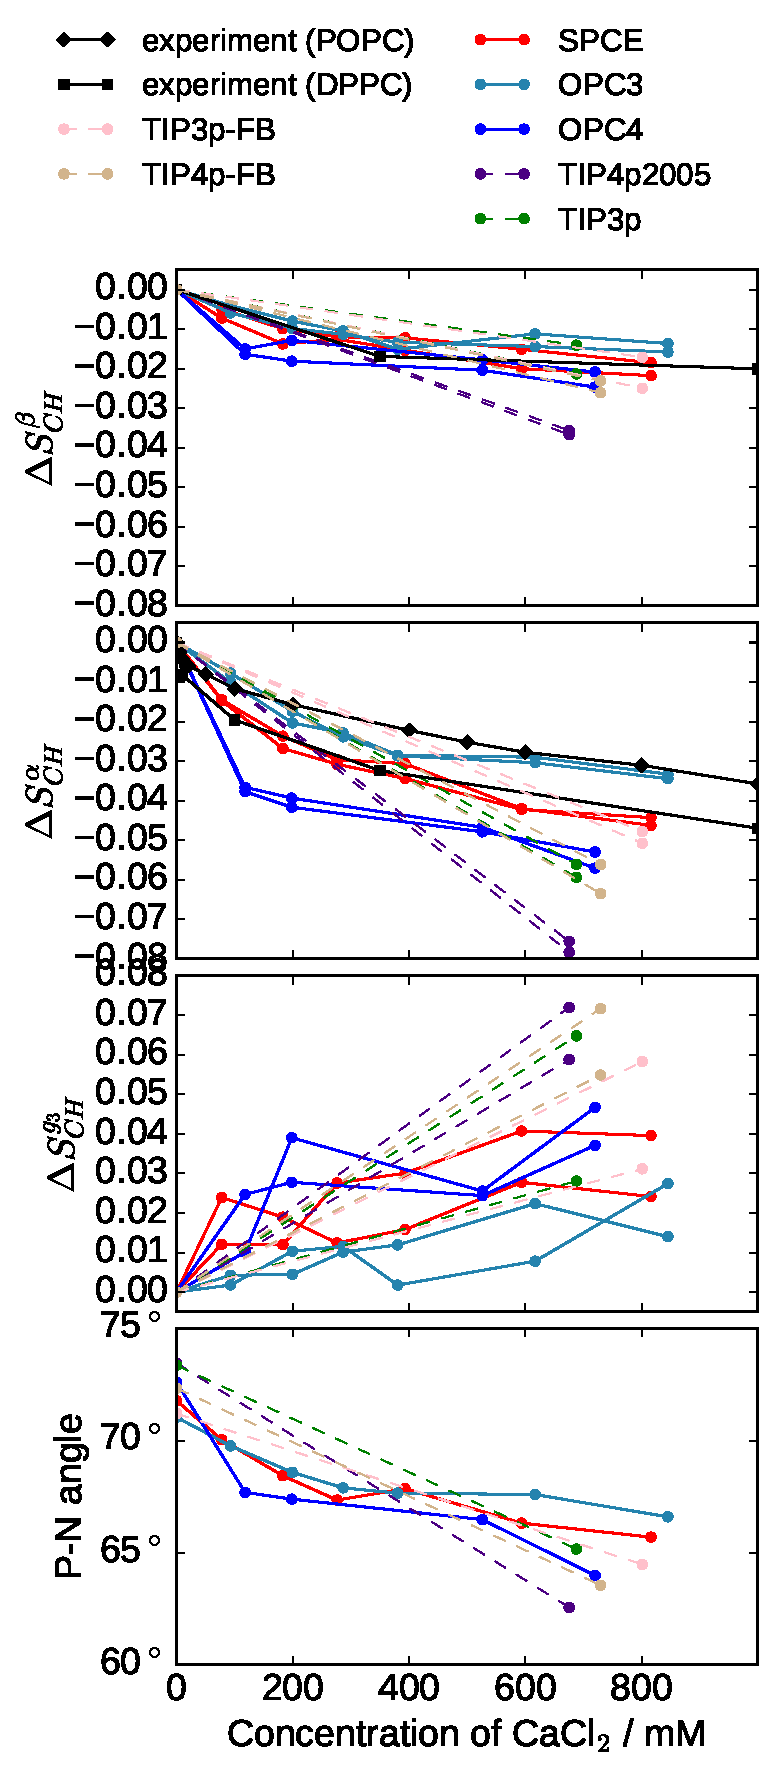
\includegraphics[width=8.0cm]{../Fig/ipython_nb/PN_angle_OrdPars-A-B-g3_L14-ECCL17_q80_sig89_CaCl_waterModels.pdf}
  \caption{\label{fig:ordPars_waterModels}
    Changes of head group order parameters of POPC bilayer as a function of CaCl$_2$ concentrations
    are shown from simulations with different force fields and water models together with experimental data 
    (DPPC \cite{akutsu81} and POPC \cite{altenbach84}). 
    Ion concentrations in bulk water are shown in x-axis. 
    Values from simulations are calculated from the of cation number density $C_{np}$
    from the region at the simulatin box edge with the constant ion concentration as [ion]=$C_{np}/0.602$.
  }
\end{figure}


\begin{figure}[tbp]
  \centering
  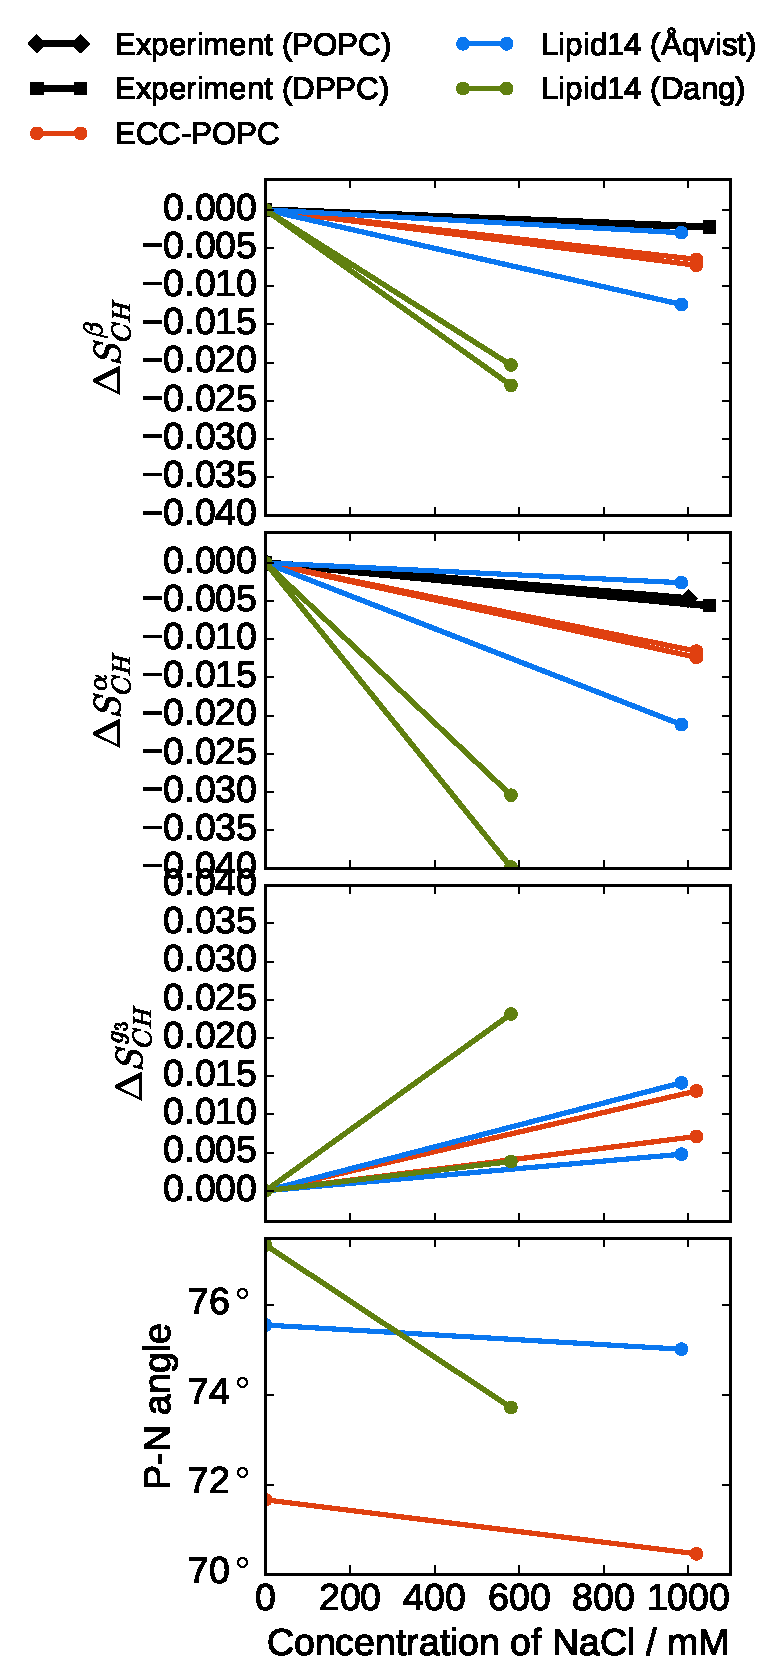
\includegraphics[width=8.0cm]{../Fig/ipython_nb/PN_angle_OrdPars-A-B-g3_L14-ECCL17_q80_sig89_NaCl.pdf}
  \caption{\label{fig:delta_ordPar_NaCl_si}
    Changes of head group order parameters of POPC bilayer as a function of NaCl concentrations
    are shown from simulations with different force fields together with experimental data \cite{akutsu81}. 
    Ion concentrations in bulk water are shown in x-axis. 
    Values from simulations are calculated from the of cation number density $C_{np}$
    from the region at the simulatin box edge with the constant ion concentration as [ion]=$C_{np}/0.602$.
    Simulation data with Lipid14 and \AA{}qvist ion parameters is taken directly from Ref. \cite{catte16}.
  }
\end{figure}



\begin{figure}[tbp!]
  \centering
  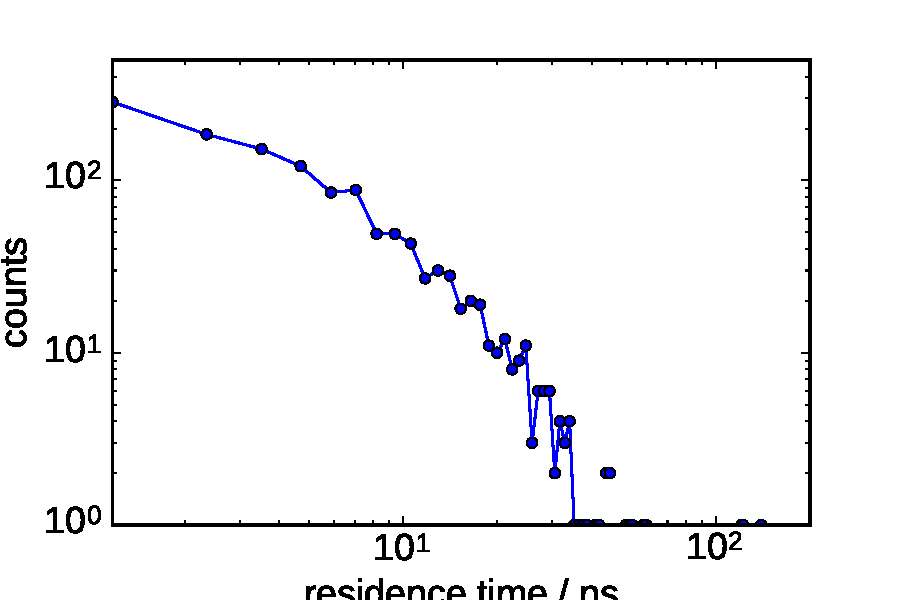
\includegraphics[width=8.0cm]{../Fig/ipython_nb/histogram_bound_times_ECC-lipids_346mM_CaCl.pdf} \\
  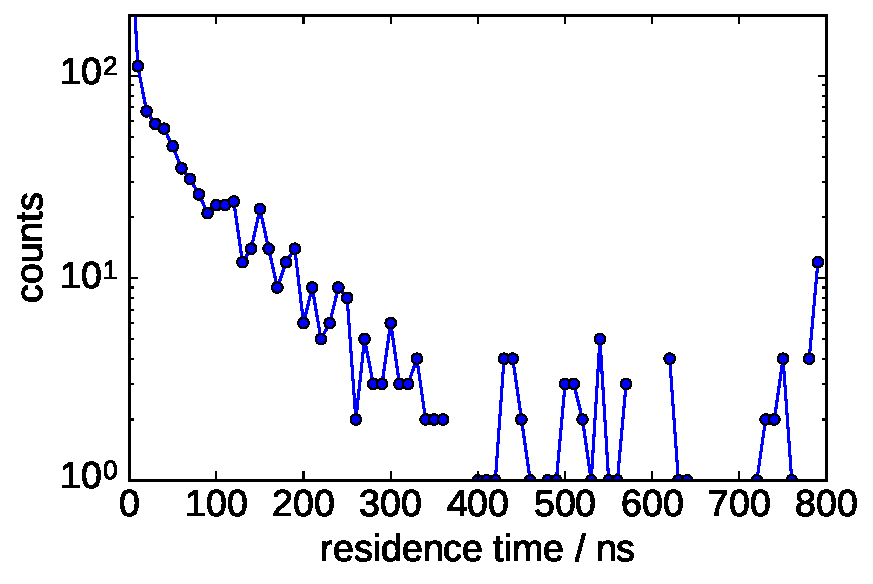
\includegraphics[width=8.0cm]{../Fig/ipython_nb/histogram_bound_times_Charmm36_450mM_CaCl_Matti.pdf}
  \caption{\label{fig:hist_residence_times}
   Histograms of residence times of \ce{Ca^{2+}} in a POPC bilayer 
   at $450\,\mathrm{mM}$ concentration of \ce{CaCl_2} in water before adsorption to phospholipids
   from simulations with ECC-lipids/ECC-ions (top)
   and CHARMM36/ECC-ions (bottom), which was taken from previous study \cite{javanainen17} 
   (simulation data available at Ref.~\citenum{zenodo.259376}).
   The maxima on the x-axis represent the lengths of the simulations used for analysis. 
   For the ECC-lipids model, 90\% of the residence times of \ce{Ca^{2+}} in a POPC membrane are 
   shorter than $60\,\mathrm{ns}$, % exactly $53\,\mathrm{ns}$
   with the longest observed residence time being $141\,\mathrm{ns}$, 
   which is well below the total length of the simulation (200~ns).
   This is, however not true for the simulation with CHARMM36 model,
   where there are several calcium cations with their residence time 
   apparently limited by the length of the simulation. 
   With such a simulation, which is relatively short for the employed model,
   we can merely estimate an upper bound that 
   only less than 60\% of the bound residence time 
   is formed by cations interacting with the phospholipid membrane 
   for less then half of the simulation length~(400~ns).
  }
\end{figure}


\begin{table}[tb!]
  \caption{Area per lipid (APL) from different models of POPC with no ions\label{tab:apls_si} }
  \begin{tabular}{l|c c}
    model          & APL (\AA$^2$)   & Temperature [K] \\
    \hline
    Lipid14                   & 65.1$\pm$ 0.6  &  300 \\
    Lipid14 \cite{dickson14}  & 65.6$\pm$ 0.5  &  303 \\
    \hline
    ECC-lipids &        &  \\
    %Lipid14ecc0.80+sigma0.875 &        &  313    \\
    %($4.6\cdot 5.1 \, \mathrm{nm}^2$), 72 lipids patch, OPC3           & 63.2   &   313      \\
    ~ OPC3           & 62.2$\pm$ 0.6   &  300       \\
    ~ OPC3           & 64.2$\pm$ 0.6   &  313       \\
    ~ SPC/E          & 65.1$\pm$ 0.6   &  313       \\
    ~ SPC/E          & 63.2$\pm$ 0.6   &  300       \\
    ~ OPC            & 64.4$\pm$ 0.6   &  313       \\
    ~ TIP4p/2005     & 66.8$\pm$ 0.6   &  313       \\
    ~ TIP3p          & 66.2$\pm$ 0.6   &  313       \\
    ~ TIP3p-FB       & 64.8$\pm$ 0.6   &  313       \\
    ~ TIP4p-FB       & 65.6$\pm$ 0.6   &  313       \\
    %($9.2\cdot 10.2 \, \mathrm{nm}^2$), 288 lipids patch           & 65.5   &  313       \\ %% not done for this model with f_sigma=0.89
    %oMM small patch           & 63.65  &         \\
    %oMM 4xbig patch           & 63.7   &         \\
    \hline
    experiment   & 62.7  &  293    \\
    experiment \cite{kucerka11} & 64.3  &  303    \\
    experiment  & 67.3  &  323    \\
    experiment  & 68.1  &  333    \\
    %experiment POPE  & 56.6 &  303    \\
    \hline
  \end{tabular} \\
\end{table}


\begin{table}[btp!]
  \caption{Simulation parameters}
  \label{tbl:mdpar}
  \begin{tabular}{ll}
    simulation property & parameter   \\
    \hline
    time-step           & 2~fs         \\
    equilibration time  & 100~ns  \\
    total simulation time     & 300~ns  \\
    temperature         & 313~K       \\
    thermostat          & v-rescale  \cite{bussi07}   \\
    barostat            & Parrinello-Rahman, semi-isotropic \cite{parrinello81} \\
    long-range electrostatics & PME  \cite{darden93}  \\
    cut-off scheme      & Verlet \cite{Pall13}      \\
    Coulomb and VdW cut-off & 1.0~nm \\
    constraints         & LINCS, only hydrogen atoms \cite{hess97} \\
    constraints for water & SETTLE  \cite{miyamoto92} \\
    \hline
  \end{tabular}
\end{table}

\begin{figure}[tbp!]
  \centering
  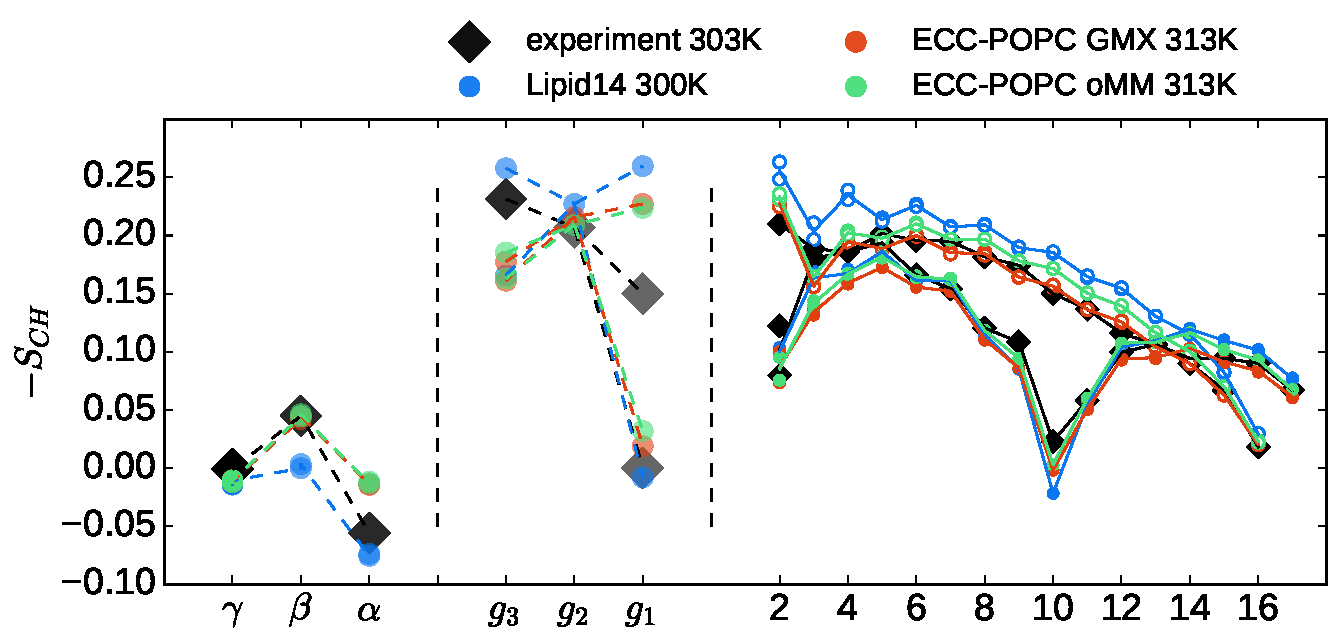
\includegraphics[width=16.0cm]{../Fig/ipython_nb/Order-parameters_exp-L14-ECCL17_q80_sig89_GMX-oMM_compar.pdf}
  \caption{\label{fig:ordPars_actual_GMX_oMM_compar}
    Order parameters of POPC head group, glycerol backbone and acyl chains 
    from simulations with the Lipid14 \cite{dickson14} and the ECC-lipids models
    simulated with GROMACS~5.1.4 \cite{Abraham15} and openMM~7 \cite{openmm7} 
    compared with the experimental values from \cite{ferreira13}.
    The size of the markers for the head group order parameters correspond to
    the error estimate $\pm 0.02$ for experiments \cite{botan15,ollila16},
    while the error estimate for simulations is $\pm 0.005$.
    The size of the points for acyl chains are decreased by a factor of 3 to improve the clarity of the plot.
  }
\end{figure}

\begin{figure}[tbp!]
  \centering
  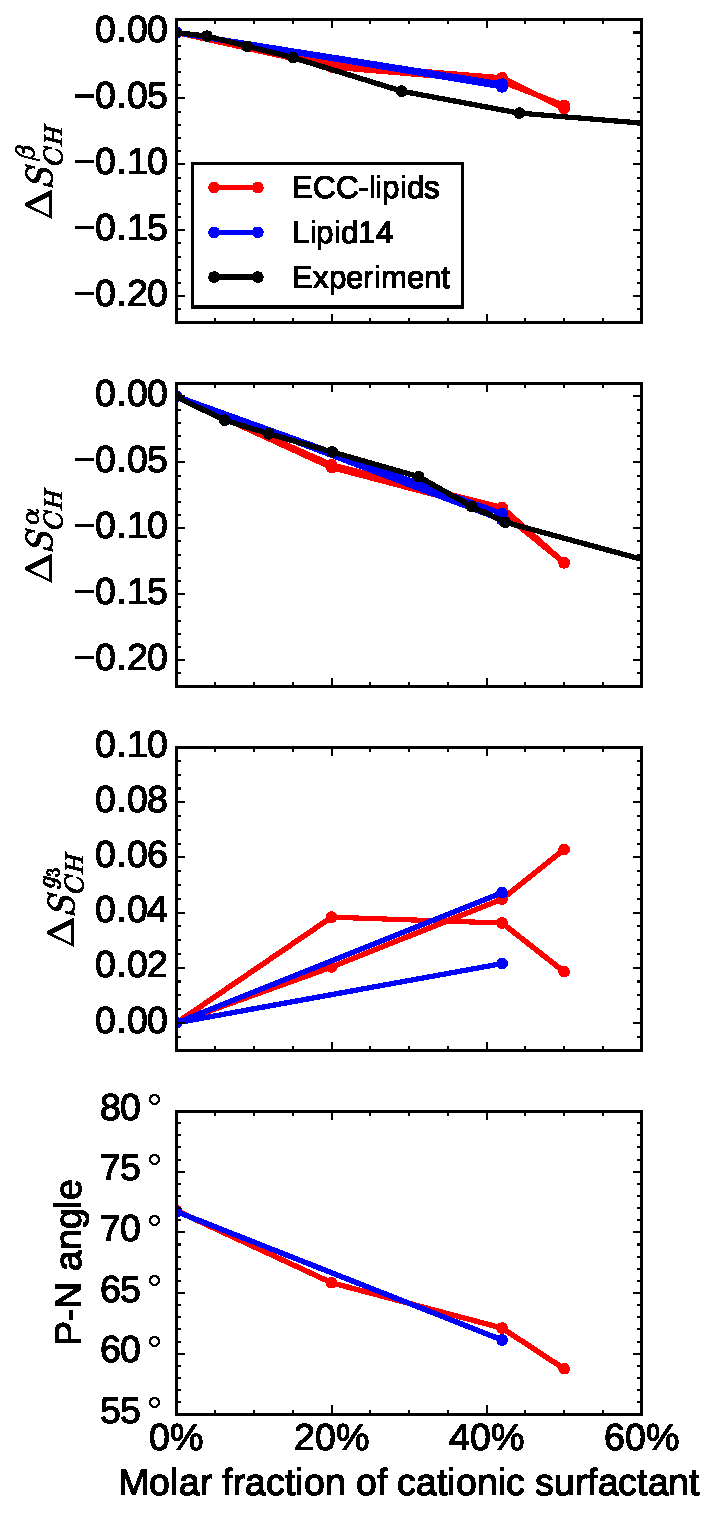
\includegraphics[width=8.0cm]{../Fig/ipython_nb/PN_angle_OrdPars-A-B-g3_L14-ECCL17_q80_sig89_surf_GMX-oMM_compar.pdf}
  \caption{\label{fig:ordPars_surf_GMX_oMM_compar}
    The changes of headgroup order parameters and P-N vector orientation as a function of
    a molar fraction of the cationic surfactant dihexadecyldimethylammonium in a POPC bilayer
    from simulations with the ECC-lipids models
    simulated with GROMACS~5.1.4 \cite{Abraham15} and openMM~7 \cite{openmm7} 
    compared with the experimental values from \cite{scherer89}.
    The size of the markers for the head group order parameters correspond to
    the error estimate $\pm 0.02$ for experiments \cite{botan15,ollila16},
    while the error estimate for simulations is $\pm 0.005$.
  }
\end{figure}

\begin{figure}[tbp!]
  \centering
  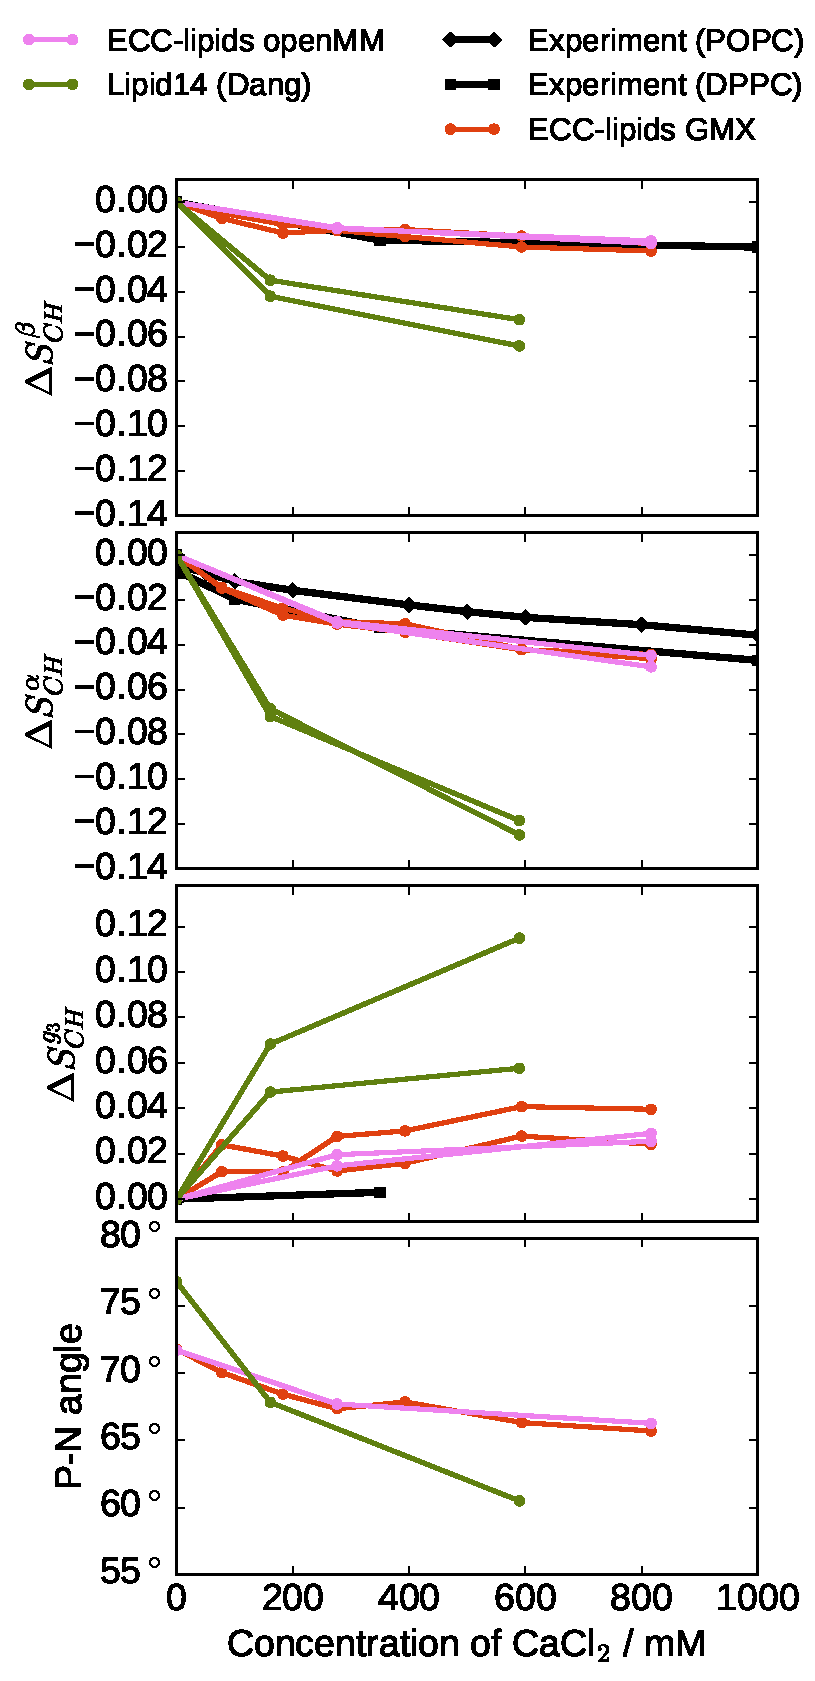
\includegraphics[width=8.0cm]{../Fig/ipython_nb/PN_angle_OrdPars-A-B-g3_L14-ECCL17_q80_sig89_CaCl_GMX-oMM_compar.pdf}
  \caption{\label{fig:ordPars_cacl_GMX_oMM_compar}
    Changes of the head group order parameters and P-N vector orientation of a POPC bilayer 
    as a function of the CaCl$_2$ concentration
    from simulations with the Lipid14 \cite{dickson14} and the ECC-lipids models
    simulated with GROMACS~5.1.4 \cite{Abraham15} and openMM~7 \cite{openmm7} 
    (DPPC (323\,K) \cite{akutsu81} and POPC (313\,K) \cite{altenbach84}). 
    Ion concentrations in bulk water are shown in x-axis. 
    Bulk concentrations from simulations are calculated 
    from the farthest point from the lipid bilayer in the aqueous phase
    with an error estimate of 10\,mM.
  }
\end{figure}

% Create the reference section using BibTe
\bibliography{refs.bib}

%\newpage
%\section{APPENDIX: The NMR results reported by Tiago Ferreira}

\listoftodos

\end{document}
%
% ****** End of file aiptemplate.tex ******
